% ---------------------------------------------------------------------------------------------------------------
% TEMPLATE PARA TRABALHO DE CONCLUSÃO DE CURSO
% Universidade Federal do Sul e Sudeste do Pará - UNIFESSPA
% Customização da classe abnTeX2 (http://www.abntex.net.br/) para as normas da UNIFESSPA/FACEEL
%
% Autor: Gilberto Pinheiro de Oliveira
%
%----------------------------------------------------------------------------------------------------------------
% Codificação: UTF-8
% LaTeX:  abnTeX2          
% ---------------------------------------------------------------------------------------------------------------

% CARREGA CLASSE abntex2 --------------------------------------------------------------------------
\documentclass[oneside]{faceel-abntex2}

% REFERÊNCIAS------------------------------------------------------------------
\usepackage[%
	alf,
	abnt-emphasize=bf,
	bibjustif,
	recuo=0cm,
	abnt-url-package=url,       % Utiliza o pacote url
	abnt-refinfo=yes,           % Utiliza o estilo bibliográfico abnt-refinfo
	abnt-etal-cite=3,
	abnt-etal-list=3,
	abnt-thesis-year=final
]{abntex2cite}	% Configura as citações bibliográficas conforme a norma ABNT

% PACOTES----------------------------------------------------------------------
\usepackage[utf8]{inputenc}                                 % Codificação do documento
\usepackage[T1]{fontenc}                                    % Seleção de código de fonte
\usepackage{booktabs}                                       % Réguas horizontais em tabelas
\usepackage{color, colortbl}                                % Controle das cores
\usepackage{float}                                          % Necessário para tabelas/figuras em ambiente multi-colunas
\usepackage{graphicx}                                       % Inclusão de gráficos e figuras
\usepackage{icomma}                                         % Uso de vírgulas em expressões matemáticas
\usepackage{indentfirst}                                    % Indenta o primeiro parágrafo de cada seção
\usepackage{microtype}                                      % Melhora a justificação do documento
\usepackage{multirow, array}                                % Permite tabelas com múltiplas linhas e colunas
\usepackage{subeqnarray}                                    % Permite subnumeração de equações
\usepackage{lastpage}                                       % Para encontrar última página do documento
\usepackage{verbatim}                                       % Permite apresentar texto tal como escrito no documento, ainda que sejam comandos Latex
\usepackage{amsfonts, amssymb, amsmath}                     % Fontes e símbolos matemáticos
\usepackage[algoruled, portuguese]{algorithm2e}             % Permite escrever algoritmos em português
\usepackage{times}                                          % Usa a fonte Times
\usepackage[bottom]{footmisc}                               % Mantém as notas de rodapé sempre na mesma posição
\usepackage{ae, aecompl}                                    % Fontes de alta qualidade
\usepackage{latexsym}                                       % Símbolos matemáticos
\usepackage{lscape}                                         % Permite páginas em modo "paisagem"
\usepackage[final]{pdfpages}								% Incluir documentos PDF

% CONFIGURAÇÕES DE APARÊNCIA DO PDF FINAL--------------------------------------
\makeatletter
\hypersetup{%
	portuguese,
	colorlinks=true,   % true: "links" coloridos; false: "links" em caixas de texto
	linkcolor=black,    % Define cor dos "links" internos
	citecolor=black,    % Define cor dos "links" para as referências bibliográficas
	filecolor=black,    % Define cor dos "links" para arquivos
	urlcolor=black,     % Define a cor dos "hiperlinks"
	breaklinks=true,
	pdftitle={\@title},
	pdfauthor={\@author},
	pdfkeywords={abnt, latex, abntex, abntex2, faceel-abntex2},
	pdfcreator={LaTeX with abnTeX2},
	bookmarksdepth=4
}
\makeatother

% ALTERA O ASPECTO DA COR AZUL--------------------------------------------------
\definecolor{blue}{RGB}{41,5,195}

% CRIA ÍNDICE REMISSIVO---------------------------------------------------------
\makeindex

% HIFENIZAÇÃO DE PALAVRAS QUE NÃO ESTÃO NO DICIONÁRIO---------------------------
\hyphenation{%
	qua-dros-cha-ve
	Kat-sa-gge-los
}

% INCLUI O PREÂMBULO DO DOCUMENTO
%
% Documento: PREÂMBULO
%

\instituicao{UNIVERSIDADE FEDERAL DO SUL E SUDESTE DO PARÁ \\ 
				INSTITUTO DE GEOCIÊNCIAS E ENGENHARIAS}
\abreviatura{UNIFESSPA}
\departamento{Faculdade de Computação e Engenharia Elétrica}
\local{Marabá-PA}
\programa{Bacharelado em Sistemas de Informação}
\nomeautor{Gilberto Pinheiro de Oliveira}
\titulotb{Projeto e Implementação de Partes Componentes de um Jogo Educativo Lúdico com Tema Histórico Sobre a Guerrilha do Araguaia}
%\subtitulo{Sub-título (se houver)}
\data{2018}
\grau{Bacharel em Sistemas de Informação}
\dataapresentacao{27 de julho de 2018}

% Dados Orientador
\orientador{Manoel Ribeiro Filho}
\titulacaoorientador{Prof. Dr.}
\instOrientador{FACEEL/UNIFESSPA}
\departamentoorientador{FACEEL}

% Dados Coorientador
\coorientador{}
\titulacaocoorientador{}
\instCoorientador{}
\departamentocoorientador{}

% Dados Examinador 1
\nmexamum{Maria Eliane Sobrinho}
\instexamum{CTIC/UNIFESSPA}
\departamentoexamum{CTIC}
\titulacaoexamum{Tec. Ma.}

% Dados Examinador 2
\nomeexamdois{Zenaide Carvalho da Silva}
\instexamdois{FACEEL/UNIFESSPA}
\departamentoexamdois{FACEEL}
\titulacaoexamdois{Prof. Dra.}

\begin{document}
	
 	% Retira espaço extra obsoleto entre as frases.
	\frenchspacing

	% Elementos pré textuais
	\pretextual
	%
% CAPA
%

\makeatletter
\begin{capa}
	\thispagestyle{empty} % Limpa estilo da pagina
	\setlength{\baselineskip}{1.2\baselineskip}
	\begin{center} % Alinhamento centralizado
		\textbf{\expandafter\uppercase\expandafter{\imprimirinstituicao}}\\
		\textbf{\expandafter\expandafter{\imprimirdepartamento}}\\
		\textbf{\expandafter\expandafter{\imprimirprograma}}\\
		\vspace*{4.55cm} % Espaçamento entre linhas
		\textbf{\expandafter\expandafter{Trabalho de Conclusão de Curso}}\\
		\vspace*{4.1cm} % Espaçamento entre linhas
		\textbf{\expandafter\uppercase\expandafter{\imprimirtitulotb}}\\
		\abntex@ifnotempty{\imprimirsubtitulo} {%
			\textbf{\expandafter\expandafter{\imprimirsubtitulo}}\\
		}
		\vspace*{4.7cm} % Espaçamento entre linhas	
		\textbf{\expandafter\expandafter{\imprimirnomeautor}}\\
		\vspace*{3.7cm} % Espaçamento entre linhas
		\textbf{\expandafter\expandafter{\imprimirlocal}} \\
		\textbf{\expandafter\expandafter{\imprimirdata}} \\
	\end{center} %Alinhamento centralizado
\end{capa}
\makeatother



 % Capa
	%
% Documento: FOLHA DE ROSTO
%

\makeatletter
\begin{folhaderosto}
	\thispagestyle{empty} % Limpa estilo da pagina
	\setlength{\baselineskip}{1.2\baselineskip}
	\begin{center}
		
		\textbf{\expandafter\expandafter{\imprimirnomeautor}}\\
		\vspace*{5.1cm} % Espaço entre linhas
		\textbf{\expandafter\uppercase\expandafter{\imprimirtitulotb}}\\
		\abntex@ifnotempty{\imprimirsubtitulo} {%
			\textbf{\expandafter\expandafter{\imprimirsubtitulo}}\\
		}
		
	\end{center}
	
	\vspace*{4.38cm} % Espaçamento entre linhas
	\hfill % Estica horizontamente  com espaços
	\begin{minipage}{8cm} % Minipagina
		\begin{normalsize} % Muda tamanho da fonte
			\setlength{\baselineskip}{0.78\baselineskip}
			
			{Trabalho de Conclusão de Curso, apresentado à Universidade Federal do Sul e Sudeste do Pará, como parte dos requisitos necessários para obtenção do Título de \imprimirgrau.}\\{
			}\\\textbf{Orientador:}\\{\imprimirtitulacaoorientador }{ }{\imprimirorientador}\\{
			}%\textbf{Coorientador:}\\{\imprimirtitulacaocoorientador }{ }{\imprimircoorientador}
			
		\end{normalsize} % Muda tamanho da fonte
	\end{minipage} % Minipagina
	
	\vspace*{5.9cm} % Espaçamento entre linhas
	
	\begin{center} % Alinhamento centralizado
		\normalsize % Muda tamanho da fonte
		\textbf{\imprimirlocal}\\
		\textbf{\imprimirdata}
	\end{center}%Alinhamento centralizado
	
\end{folhaderosto}
\makeatother % Folha de rosto
	% FICHA CATALOGRÁFICA ------------------------------------------------------------------------
\includepdf[pages=-]{figuras/FichaCatalografica.pdf}
% FIM % Ficha catalográfica
	% FOLHA DE APROVAÇÃO ------------------------------------------------------------------------
\includepdf[pages=-]{figuras/FolhaAprovacao.pdf}
% FIM % Folha de aprovação
	%
% Documento: DEDICATÓRIA
%

\thispagestyle{empty}

\begin{dedicatoria}	
\textit{À minha família, por sua capacidade de acreditar em mim e investir em mim. Mãe, seu cuidado e dedicação foi que deram, em alguns momentos, a esperança para seguir. Pai, sua presença significou segurança e certeza de que nunca estive sozinho nessa caminhada.}
\end{dedicatoria} % Dedicatória
	%
% Documento: AGRADECIMENTOS
%

\begin{agradecimento}
	
	Agradeço primeiramente à Deus, por ser essencial em minha vida, autor e norteador do meu destino, meu guia, auxílio presente nos momentos mais difíceis dessa caminhada.
	
	Ao professor \imprimirorientador \space por ter acreditado em mim, por todo o conhecimento compartilhado e por ter me incentivado durante esses três anos de iniciação científica, o que possibilitou a realização deste trabalho.
	
	A todos os integrantes do Laboratório de Games Educativos (LAGE)\footnote{\url{https://lage.unifesspa.edu.br}} -- Denison Resplandes, Caíque Silva, Adriano Souza, Ernesto Neto, Tiago Araújo, Felipe Nogueira e Marcos Sobral, que possibilitaram a realização deste trabalho e me ajudaram nos momentos de dúvidas.
	
	Ao meu pai Alberto Conceição Barbosa de Oliveira que não mediu esforços para me proporcionar uma vida melhor e que foi um exemplo para mim, sempre batalhador, dedicado e esforçado.
	
	A minha mãe Maria das Graças Miranda Pinheiro que sempre esteve ao meu lado durante o desenvolvimento deste trabalho, nunca deixando eu me desviar dos meus objetivos, incentivando-me em cada momento dessa jornada.
	
	A Universidade Federal do Sul e Sudeste do Pará (UNIFESSPA), ao Programa Institucional de Bolsas de Iniciação Científica (PIBIC)\footnote{\url{http://cnpq.br/pibic}} e ao Conselho Nacional de Desenvolvimento Científico e Tecnológico (CNPQ)\footnote{\url{http://cnpq.br/}} pela oportunidade de uma bolsa de pesquisa que culminou neste trabalho.
	
	A todos os meus professores do curso Bacharelado em Sistemas de Informação pela grande contribuição na minha vida, o que possibilitou a aquisição de conhecimentos essenciais para a concretização deste trabalho.
	
	Aos familiares e amigos que direta e indiretamente me incentivaram e me apoiaram nesta jornada de quatro anos de graduação.
	
\end{agradecimento}

 % Agradecimentos
	%
% Documento: EPIGRAFE
%

\begin{epigrafe}
		
	\textit{\textbf{ Talvez não tenha conseguido fazer o melhor, mas lutei para que o melhor fosse feito. Não sou o que deveria ser, mas Graças a Deus, não sou o que era antes.}}{\\}{\\}
	
	\begin{autorepigrafe}
		\textit{\textbf{(Marthin Luther King)}}
	\end{autorepigrafe}
		
\end{epigrafe} % Epígrafe
	%
% Documento: RESUMO (Português)
%

\begin{RESUMO}
	\begin{SingleSpace}
		
	\hspace{-1.5cm}O jogo  educativo \textit{Araguaia: A Saga de Osvaldão} para a plataforma \textit{mobile (Android)}, começou a ser desenvolvido em agosto de $2016$ pela equipe do Laboratório de Games Educativos (LAGE) da Universidade Federal do Sul e Sudeste do Pará (UNIFESSPA), com o intuito de transformar uma narrativa histórica regional -- Guerrilha do Araguaia -- em um game educativo idealizado para ser utilizado como ferramenta auxiliar no processo de ensino-aprendizagem da disciplina de História para turmas do ensino médio das escolas de Marabá-PA. O enredo do jogo foi construído na atuação do guerrilheiro Osvaldão, pois este teve um papel muito importante na Guerrilha. O projeto do jogo prevê duas fases -- \textit{$1ª$ fase: período de inserção de Osvaldão e seus companheiros guerrilheiros na região do ``Bico do Papagaio"\space $(1966-1971)$; e $2ª$ fase: período de combate da Guerrilha $(1972-1974)$}. Cada uma delas é constituída por \textit{cutsecenes} e missões. Este trabalho apresenta o projeto e implementação, de uma \textit{cutscene} em \textit{3D}, três \textit{cutscenes} em \textit{2D} e de quatro missões, duas primeiras relacionadas a primeira fase, e duas a segunda fase. Os cenários, objetos e personagens foram modelados por outros membros da equipe do LAGE. A \textit{cutscene} \textit{3D} foi concebida usando o software \textit{Blender}, para a modelagem tridimensional do ambiente, e o software \textit{Makehuman}, para a criação dos personagens humanoides. As \textit{cutscenes 2D} foram implementadas utilizando a \textit{Unity} -- motor de desenvolvimento integrado que fornece funcionalidades pioneiras para a criação de jogos e outros conteúdos interativos. As quatro missões supracitadas também foram implementadas utilizando a \textit{Unity}. Posteriormente, o jogo foi avaliado pela equipe e apresentado para alunos de uma escola de Marabá-PA, obtendo resultados animadores.
	
	\vspace*{0.5cm}\hspace{-1.5 cm}\textbf{Palavras-chave}: Jogo educativo. Plataforma \textit{2D}. Guerrilha do Araguaia. Osvaldão.
	
	\end{SingleSpace}
\end{RESUMO} % Resumo
	%
% Documento: RESUMO (Inglês)
%

\begin{ABSTRACT}
	\begin{SingleSpace}
				
		\hspace{-1.5cm}The educational game \textit{Araguaia: The Saga of Osvaldão} for the mobile platform (Android), began to be developed in august of $2016$ by the team of the Laboratório de Games Educativos (LAGE) of the Universidade Federal do Sul e Sudeste do Pará (UNIFESSPA), with the purpose of transforming a regional historical narrative -- Araguaia's Guerrilla -- into an educational game idealized to be used as an auxiliary tool in the teaching-learning process of the History discipline for high school classes schools in Marabá-PA. The story of the game was built in the action of the guerrilla Osvaldão, because this had a very important role in the Guerrilla. The project of the game provides for two phases -- \textit{$1st$ phase: period of insertion of Osvaldão and his companions guerrillas in the region of ``Bico do Papagaio"\space $(1966-1971)$; and $2nd$ phase: a battle period of Guerrilla $(1972-1974)$}, each consisting of cutscenes and missions. This paper presents the design and implementation of a one cutscene in 3D, three cutscenes in 2D and four missions, two first related to the first phase, and two the second phase. The scenarios, objects and characters were modeled by other members of the LAGE team. The cutscene 3D was designed using the Blender software, for the three-dimensional modeling of the environment, and the Makehuman software, for the creation of humanoid characters. The cutscenes 2D were implemented using the Unity -- development engine that provides pioneering features for creating games and other interactive content. The four missions mentioned above were also implemented using Unity. Later, the game was evaluated by the team and presented to students of a school in Marabá-PA, obtaining encouraging results.
		
		\vspace*{0.5cm}\hspace{-1.5 cm}\textbf{Keywords}: Educational Game. 2D Plataform. Araguaia's Guerrilla. Osvaldão.
				
	\end{SingleSpace}
	
\end{ABSTRACT}
 % Abstract
	%
% Documento: LISTA DE FIGURAS
%

\pdfbookmark[0]{\listfigurename}{lof}
\listoffigures*
\cleardoublepage % Lista de Figuras
	\include{01-pre-textuais/lista-tabelas} % Lista de Tabelas
	%
% Documento: LISTA DE ABREVIATURAS E SIGLAS
%

\begin{siglas}
	\setlength{\baselineskip}{0.7\baselineskip}
	
	\item[CNPQ] Conselho Nacional de Desenvolvimento Científico e Tecnológico
	\item[PIBIC] Programa Institucional de Bolsas de Iniciação Científica
	\item[PIBEX] Programa Institucional de Bolsas de Extensão
	\item[UNIFESSPA] Universidade Federal do Sul e Sudeste do Pará
    \item[LAGE] Laboratório de Games Educativos
    \item[\textit{2D}] \textit{Two Dimensions}
    \item[\textit{3D}] \textit{Three Dimensions}
    \item[Abragames] Associação Brasileira dos Desenvolvedores de Jogos Digitais
    \item[SBGames] Simpósio Brasileiro de Jogos e Entretenimento Digital
    \item[\textit{GDD}] \textit{Game Design Document}
    \item[\textit{ADDIE}] \textit{Analyze, Design, Develop, Implement and Evaluate}
    \item[\textit{NaN}] \textit{Not a Number}
    \item[\textit{GNU}] \textit{GNU is Not Unix}
    \item[\textit{GPL}] \textit{General Public License}
    \item[\textit{SVG}] \textit{Scalable Vector Graphics}
    \item[\textit{W3C}] \textit{World Wide Web Consortium}
    \item[\textit{XML}] \textit{eXtensible Markup Language}
    \item[\textit{GIMP}] \textit{GNU Image Manipulation Program}
    \item[\textit{C$\sharp$}] \textit{C Sharp}
    \item[\textit{RPG}] \textit{Role-Playing Game}
    \item[\textit{FPS}] \textit{First Person Shooter}
    \item[\textit{PC}] \textit{Personal Computer}
    \item[\textit{iOS}] \textit{iPhone Operating System}
    \item[TCC] Trabalho de Conclusão de Curso
    \item[PCdoB] Partido Comunista do Brasil
    \item[\textit{HUD}] \textit{Heads-up Display}
    \item[SBIE] Simpósio Brasileiro de Informática na Educação
\end{siglas} % Lista de Abreviaturas e Siglas
	\sumario % Sumário
	
	% Elementos textuais
	\textual
	% INTRODUÇÃO-------------------------------------------------------------------

\chapter{INTRODUÇÃO}
\label{chap:introducao}

O número de desenvolvedores de games no Brasil vêm crescendo nos últimos anos. Segundo pesquisa realizada pela Associação Brasileira dos Desenvolvedores de Jogos Digitais (Abragames), enquanto o setor de serviços no país tem sofrido quedas consecutivas, um nicho prospera em tendência oposta. Trata-se do mercado de produção de jogos virtuais. Em oito anos, o número de empresas desenvolvedoras de games aumentou em quase $600\%$. Já o faturamento do setor no país cresceu $25\%$ entre $2014$ e $2016$ \cite{bib:globo2017}.

Um outro levantamento feito pela \textit{NewZoo}, uma das principais condutoras de pesquisas sobre a indústria dos games no mundo, mostra que em $2016$ o setor faturou $US\$ 1,6$ bilhão no Brasil, um aumento de $25\%$ em relação a 2014, quando o mercado brasileiro de jogos digitais movimentou $US\$ 1,28$ bilhão \cite{bib:globo2017}.

Entretanto, segundo Raoni Dorim, sócio da empresa \textit{Mopix Games}\footnote{http://www.mopix.com.br}, a produção de jogos digitais não se restringe ao propósito de entretenimento. Um dos nichos com grande potencial de crescimento é o de \textit{serious} games, ou jogos empresariais, que engloba jogos educativos e simuladores \cite{bib:globo2017}.

Aproveitando este potencial de crescimento registrado, o objeto de estudo deste trabalho são os jogos eletrônicos educativos, que propõem a seguinte premissa: tentar auxiliar um educador no ensino de um conteúdo, de forma lúdica e divertida, aumentando a motivação dos participantes, contribuindo positivamente para o processo ensino-aprendizagem \cite{bib:tori2010}.

O desenvolvimento de jogos digitais pode ser considerado como uma tarefa complexa, que exige uma gama de conhecimentos técnicos nas mais diversas áreas, desde a programação de computadores até o conhecimento artístico para o preparo de elementos, sejam eles gráficos ou escritos \cite{bib:bb2016}.

Dentre os elementos considerados essenciais em um jogo eletrônico educativo estão as \textit{cutscenes} -- cena que desenvolve a linha narrativa e é costumeiramente mostrada no momento que algum nível do jogo é completado ou iniciado \cite{bib:cs2016}. Geralmente, neste tipo de cena, não há interação entre jogador e personagem, caracterizando-a como uma narrativa de fluxo linear.

O jogo educativo ``Araguaia: A Saga de Osvaldão", até o momento possui cinco \textit{cutscenes}, uma em \textit{3D} e o restante em \textit{2D}. A \textit{3D} foi concebida com o auxilio de softwares \textit{open-source} para modelagem tridimensional de cenários e personagens, produção e edição de vídeo e animação de objetos \textit{3D}. As \textit{2D} foram concebidas utilizando a game \textit{engine Unity}, com o auxilio de softwares de edição de vídeo. Este trabalho apresenta o projeto e implementação da \textit{cutscene 3D} e de três \textit{cutscenes 2D}.

Além das \textit{cutscenes}, as missões \textit{(levels)} também são elementos essenciais em um game, definidas por um conjunto de regras que descrevem as etapas (desafios) necessárias para alcançar um determinado objetivo dentro do jogo. \textit{Level design} é o processo de desenvolvimento delas, nele são detalhados os desafios e missões que o jogador precisa cumprir para vencer. Os artistas trabalham na programação visual e nos cenários de cada \textit{level}, enquanto os programadores programam suas características \cite{bib:ribeiro2013}.

Neste trabalho serão apresentadas quatro missões. Duas referentes a $1ª$ fase do jogo, retratando a criação do Destacamento $B$ da Guerrilha, do qual Osvaldão era o comandante e a expulsão de um grileiro da região, feita pelo Osvaldão. E duas referentes a $2ª$ fase do jogo -- a primeira inicia relatando o processo de interação entre Osvaldão e os demais guerrilheiros com a população da região do conflito (realizando atividades em conjunto, limpando terreno e etc.) e a segunda missão mostra uma passagem que relata um encontro ocorrido às margens do rio Gameleira, entre os guerrilheiros e tropas do exército, com a participação de Osvaldão. Estas foram programadas utilizando a \textit{Unity} -- motor de desenvolvimento integrado que fornece funcionalidades pioneiras para a criação de jogos e outros conteúdos interativos.

Após a implementação destas missões, o jogo foi avaliado pela equipe do projeto e distribuído para a plataforma \textit{mobile (Android)}, deixando-o disponível para \textit{download} no site do LAGE. A avaliação pela equipe foi dividida em dois momentos: o primeiro foi a avaliação técnica, onde os membros testaram o jogo, objetivando encontrar erros de implementação das regras do jogo, bem como de \textit{bugs} de interação/experiência do usuário (demora na resposta dos botões, travamento de \textit{cutscenes} e etc). O segundo momento fora a avaliação pedagógica, onde os membros da equipe responsáveis por definir os objetivos pedagógicos do jogo avaliaram este, evidenciando se ele realmente está de acordo com o planejado, no que tange a maneira como é passado o conteúdo a ser aprendido.

\section{Motivação}
\label{sec:motivacao}

Games sobre história têm sido uma temática muito explorada em todo o mundo. Em vez de uma monografia e a apresentação de uma narrativa linear da história, o trabalho do historiador poderia ser produzido como um game. Podendo apresentar pesquisas originais que rivalizam com qualquer excelente trabalho de história, transformando leitores, estudantes e espectadores em jogadores que interagem com a história, imersos no palco dos acontecimentos. O videogame oferece um potencial muito maior para a criação e apresentação do conteúdo histórico que qualquer outro entretenimento ou mídia interativa \cite{bib:spring2015}.

Portanto, contar a história tem sido, e continua sendo um tema importante para os desenvolvedores de games, tanto no aspecto educativo como no da diversão, ou seja, tornar a narrativa lúdica e divertida ao mesmo tempo que educa e auxilia no processo de ensino-aprendizagem.

Além disso, a busca por novos métodos de ensinar história é uma motivação recorrente, e os jogos aparecem como uma ferramenta pedagógica capaz de contribuir para a aprendizagem dos conteúdos históricos e transpor algumas dificuldades encontradas no cotidiano das salas de aula. Deste modo, uso de jogos é uma prática docente que se desenvolve e é fruto de uma reflexão sobre as experiências vividas em sala de aula \cite{bib:teixeira2016}.

Assim, este trabalho traz um grande desafio, pois como transformar uma narrativa histórica em um game divertido e que ao mesmo tempo ensine ao jogador fatos políticos e históricos além de mostrar a flora e fauna da região da Guerrilha do Araguaia?

Para tanto, foi formada uma equipe multidisciplinar com historiadores, game \textit{designers}, artistas e programadores que de maneira colaborativa projetaram e implementaram, a primeira e a segunda fase de um jogo de plataforma \textit{2D} sobre a Guerrilha do Araguaia, com foco na atuação do guerrilheiro Osvaldão.

Ademais, grande parte das escolas públicas do município de Marabá-PA possuem um parque computacional pobre, em termos de recursos computacionais para executar jogos eletrônicos. Sabendo disso, este projeto entrega uma versão \textit{mobile} do software proposto à comunidade, fazendo com que os professores possam utilizá-lo em sala de aula, necessitando apenas dos \textit{smartphones} dos estudantes.

\section{Objetivo Geral}
\label{sec:objetivogeral}

Desenvolver um jogo educacional de plataforma \textit{2D} sobre a temática da Guerrilha do Araguaia $(1972-1974)$, com foco na atuação do guerrilheiro Osvaldão, idealizado como ferramenta auxiliar no processo de ensino-aprendizagem da disciplina de História em turmas do ensino médio nas escolas de Marabá-PA.

\section{Objetivos Específicos}
\label{sec:objetivosespecificos}

\begin{itemize}
		
	\item Apresentar o projeto e implementação de duas missões da primeira fase do jogo, que são: a primeira missão, construção do primeiro barracão na região do Destacamento $B$ da Guerrilha, realizada por Osvaldão. A segunda, apresenta o um episódio pouco conhecido na região, onde Osvaldão expulsou um Grileiro\footnote{Pessoa que se apodera ou procura se apossar de terras alheias, mediante falsas escrituras de propriedade} conhecido como Pedro Mineiro que, juntamente com seus capangas, oprimiam uma família de camponeses;
			
	\item Projetar e implementar duas missões da segunda fase do jogo, que são: a primeira missão, relacionamento dos guerrilheiros com a população local da região. A segunda, apresenta o primeiro conflito armado entre guerrilheiros e tropas do exército, com a participação de Osvaldão;
	
	\item Apresentar o projeto e implementação de quatro \textit{cutscenes} para o jogo, uma em \textit{3D} e três em \textit{2D};
				
	\item Aprender técnicas de projeto e implementação de jogos eletrônicos educativos de plataforma \textit{2D};
	
	\item Realizar submissão de artigos em congressos das áreas de jogos eletrônicos e informática na educação.
	
\end{itemize}

\section{Organização do Trabalho}
\label{sec:organizacaotrabalho}

O trabalho está estruturado em cinco capítulos. Os tópicos abaixo descrevem subsequentemente a organização destes.

\begin{itemize}
			
	\item \textbf{Capítulo \ref{chap:fundamentacao-teorica}:} Apresenta a fundamentação teórica deste trabalho, discutindo sobre games e educação, jogos de plataforma \textit{2D} e jogos no ensino de história. Também são apresentados três trabalhos correlatos que embasaram esta pesquisa;
	
	\item \textbf{Capítulo \ref{chap:metodologia}:} Apresenta a metodologia empregada para a realização deste trabalho, onde destacam-se o \textit{Game Design Document (GDD)}; o \textit{Framework} de desenvolvimento de jogos educativos elaborado pela equipe e empregado neste projeto; as ferramentas de desenvolvimento de jogos utilizadas; e as especificações técnicas usadas para o desenvolvimento do jogo e para definir os requisitos mínimos da plataforma de execução deste;
	
	\item \textbf{Capítulo \ref{chap:araguaia-osvaldao}:} Apresenta a ambientação da equipe do projeto, no âmbito da Guerrilha do Araguaia; o projeto do jogo; a implementação das duas missões da primeira fase, bem como das duas da segunda fase; a implementação das quatro \textit{cutscenes}, sendo três na primeira fase e uma na segunda fase; e as avaliações do jogo, dando um destaque para a avaliação técnica e a pedagógica;
	
	\item \textbf{Capítulo \ref{chap:conclusao}:} Expõe as considerações finais acerca do trabalho realizado. Nela tem-se os resultados alcançados com a implementação das duas fases do jogo, bem como perspectivas de trabalhos futuros, dando um destaque para a realização de avaliações com alunos sobre o jogo.
	
\end{itemize} % Introdução
	% REVISÃO DE LITERATURA--------------------------------------------------------

\chapter{REVISÃO DE LITERATURA}
\label{chap:fundamentacao-teorica}

Neste capítulo será descrito o referencial teórico que embasou esta pesquisa. Descrevendo a relação entre games e educação; comentando sobre jogos de plataforma \textit{2D} e jogos no ensino de História. Também apresentando três trabalhos correlatos (artigos publicados no SBGames) que apresentam jogos educativos para o ensino de História.

\section{Games e Educação}
\label{sec:gameseeducacao}

Com o aumento exponencial do uso de tecnologia em todas as idades, o acesso a informações se tornou muito fácil, surgiram novas formas de agir e pensar. Um profissional capaz de se reinventar de acordo com as necessidades do momento se tornou mais desejado do que um profissional que sempre age da mesma forma, que nunca está disposto a mudar. Essa nova dinâmica do mercado fez com que o modelo de ensino das escolas fosse questionado, pois aquele padrão onde o professor simplesmente transmite as informações e os alunos as decoram ficou defasado e desmotivador. Agora é necessário que os alunos aprendam a aprender, que sejam capazes de construir novos conhecimentos a partir das informações disponíveis \cite{bib:medeiros2012}.

Um jogo pode ser definido como ``um sistema no qual os jogadores se envolvem em um conflito artificial, definido por regras, que implica um resultado quantificável"\space\cite{bib:salen2012}. Já os jogos educacionais são aqueles criados para ensinar com diversão. São desenvolvidos para fins pedagógicos e geralmente contam com as crianças como público alvo. Contudo, todos os tipos de jogos permitem a obtenção de conhecimentos do mundo real pelos jogadores e muitos jogos eletrônicos são educativos por ``acidente"\space\cite{bib:novak2010}.

\citeonline{bib:medeiros2012} encorajam o uso de jogos na educação, afirmando que, além de serem fontes de diversão, os jogos podem ser utilizados para vários fins educativos e como instrumentos de desenvolvimento de crianças e jovens. Os autores explicam que, para as crianças, o jogo constitui um fim, onde o objetivo principal é a diversão. Já para os educadores, o jogo é um meio, um veículo que permite transmitir uma mensagem educativa de forma atraente e prazerosa, cabe ao professor escolher o jogo que melhor se aplica ao conteúdo que deseja ensinar.

Com o desenvolvimento tecnológico, surgiu uma nova modalidade de jogos, os eletrônicos, mas a utilização desse tipo de jogo na área da educação ainda sofre preconceitos, pois muitas vezes ele é visto como uma perda de tempo, algo que os jovens acabam se viciando e que não os ensina nada \cite{bib:medeiros2012}.

Jogos eletrônicos educacionais atuam diretamente na necessidade de romper com o atual paradigma da educação, levando-se em consideração: A importância da interatividade para manter a atenção do estudante; o desenvolvimento de um ambiente sem riscos no qual o aluno possa testar os seus conhecimentos; e a individualidade de cada aprendiz, uma vez que cada um pode aprender de forma diferenciada, assimilando conhecimentos e experiências em seu próprio ritmo \cite{bib:medeiros2012}.

\section{Jogos de Plataforma \textit{2D}}
\label{sec:plataforma2D}

Na década de $1980$ surgiram os primeiros jogos plataforma de ação e aventura, \textit{Donkey Kong}\footnote{\url{http://pt-br.donkey-kong-country.wikia.com/wiki/Donkey\_Kong(personagem)}} e \textit{Mario}\footnote{\url{http://desciclopedia.org/wiki/Mario\_(personagem)}} eram personagens que apresentavam mecânicas de interação em duas dimensões \textit{(2D)}. Os jogadores podiam andar para a direita, esquerda e para baixo e executar ações de pular, subir em escadas e atacar. Já nos anos $90$, com o desenvolvimento das tecnologias de computação, surgiram os jogos em três dimensões \textit{(3D)}. \textit{Wolfenstein 3D}\footnote{\url{http://wolf3d.atw.hu/}} e \textit{Doom}\footnote{\url{desciclopedia.org/wiki/Doom}} revolucionaram a história dos videogames por serem os primeiros jogos do gênero de tiro em primeira pessoa que apresentaram uma movimentação tridimensional semelhante ao mundo real, davam cinco graus de liberdade aos jogadores e tinham texturas consideradas realistas para a época, mas exigiam mais poder de processamento dos computadores ou videogames \cite{bib:lopes2016}.

Considerando os avanços da indústria dos jogos digitais e das tecnologias computacionais, pode-se afirmar que consoles, videogames portáteis, computadores, \textit{smartphones} e \textit{tablets} da atualidade são capazes de processar jogos com gráficos \textit{3D}. Desta forma, escolher entre fazer um jogo \textit{2D} ou \textit{3D} é de responsabilidade dos \textit{designers} de jogos e a escolha é feita através de suas propostas de jogabilidade e da preferência do seu público alvo pelo estilo de jogo.

No decorrer dos anos as desenvolvedoras adaptaram suas franquias de acordo com a melhoria das tecnologias. Jogos que surgiram na época do \textit{2D} como \textit{Prince of Persia}\footnote{\url{https://classicreload.com/prince-of-persia.html}}, \textit{Super Mario} e \textit{Castlevania}\footnote{\url{castlevania.wikia.com/wiki/Games}}, acompanharam a evolução e ganharam versões tridimensionais. Em contraponto, algumas franquias da atualidade que surgiram na era tridimensional como \textit{Assassin’s Creed}\footnote{\url{https://www.ubisoft.com/en-gb/game/assassins-creed}} e \textit{Mirro's Edge}\footnote{\url{www.mirrorsedge.com/pt\_BR/}} tomaram o caminho inverso e criaram versões com duas dimensões. Com características e interações parecidas, mas com diferenças de jogabilidade por causa das três ou duas dimensões, nem todos os jogos das franquias citadas acima agradaram $100\%$ dos fãs. Estudar as percepções dos usuários sobre executar interações em jogos com mecânicas \textit{2D} e \textit{3D} permite que sejam identificados os pontos específicos de interesse dos jogadores, os problemas que dificultam a execução das interações em cada modo de jogo e o equilíbrio necessário entre a diversão e o desafio \cite{bib:lopes2016}.

\section{Jogos no Ensino de História}
\label{sec:gameshistoria}

A História tem sido há alguns anos a fonte que retroalimenta os enredos de peças teatrais, obras literárias, filmes, novelas, histórias em quadrinhos, animes, games etc. Essa parceria no caso do cinema, data mais de um século e, até hoje, alguns títulos considerados clássicos são indicados ou exibidos nas salas de aula para promover aprendizagens, como exemplo: Danton: o processo da revolução $(1982)$, O Nome da Rosa $(1986)$, $1492$ -- A Conquista do Paraíso $(1992)$, A lista de \textit{Schindler} $(1993)$, dentre outros. Já na mídia televisiva brasileira o resultado da aproximação com a História ficou conhecido como ``trabalhos de época", aparecendo apenas na década de $70$, lançando sucessos de audiência conhecidos nacionalmente e, em alguns casos, internacionalmente tais como: Escrava Isaura $(1970)$, Sinhá Moça $(1986)$ e etc \cite{bib:neves2012}.

O uso da História pelos jogos digitais seguiu o mesmo caminho dessas duas mídias, aliando conteúdos históricos e ficção o que possibilitava não apenas a visualização, mas também a interação, ou até mesmo, a imersão nos ambientes simulados. Cabe aqui ressaltar, que, antes mesmo de ser utilizada nos jogos com formato digital, a História já era utilizada como fonte dos jogos no formato ``analógico"\space(conhecidos também como jogos de tabuleiro). Destacam-se, entre esses jogos: \textit{War} $(1972)$, \textit{Yatzi} $(1983)$, Cabral: descobrimento e criação $(2000)$, Alexander $(2003)$, \textit{Age of Heroes} $(2003)$, \textit{Angus} -- Batalhas Medievais $(2004)$, \textit{Band of Heroes} $(2005)$, Conquistadores $(2006)$, \textit{War} Império Romano $(2007)$ dentre outros \cite{bib:neves2012}.

Os acontecimentos e fatos históricos tiveram suas primeiras aparições nos jogos digitais do tipo \textit{Role-Playing Game (RPG)}, que começaram a surgir durante a década de $1970$. Estes jogos contribuíram expressivamente para a compreensão de que a História poderia ser utilizada nesses suportes, assim como já acontecia em outras mídias. Tais jogos deram sua parcela de ajuda, na medida em que articulavam em seus enredos jornadas épicas para enriquecer suas narrativas (sem um caminho linear ou final pré-estabelecido) com personagens e ambientes que remetiam o jogador ao passado e a um mundo de fantasia. Dessa forma, ao incorporar narrativas, os jogos digitais transformaram a tradição narrativa visual e revolucionaram a forma como as histórias passaram a ser contadas \cite{bib:novak2010}.

A partir daí, a História marcava presença nos jogos digitais de estratégia, que, por sua vez, adotavam em seu enredo acontecimentos históricos reportando épocas passadas, como temática central ou apenas pano de fundo para construção do enredo, mesclando ficção aos fatos ``reais". Os primeiros jogos de estratégia geralmente se desenrolavam em ambiente militar, no qual o jogador tinha que gerir os recursos e a construção de diversos tipos de edifícios e unidades \cite{bib:neves2012}.

O desenvolvimento dos jogos de ficção histórica resulta de adaptações, montagens, restrições, seleções, generalizações e, até mesmo, criações espontâneas e falsificadas, que, às vezes, não guarda quaisquer relações com os acontecimentos ditos ``reais"\space -- tornando-se, assim, uma ``história de mentira"\space \cite{bib:neves2012}. Nessa lógica, simulam acontecimentos e fatos que se produzem nas e sobre as variadas dimensões da vida, no tempo e no espaço, como uma determinada sociedade, política, economia, cultura que pode ser realista ou alegórica, fidedigna ou fantasiosa, linear ou fragmentada.

Os games de História simulam e não somente representam os fatos ou acontecimentos históricos -- como fazem os artistas plásticos em suas telas, os dramaturgos em suas peças ou os cineastas em seus filmes. Esses jogos possibilitam ao jogador assumir o centro das decisões de um ambiente intencionalmente projetado com elementos históricos cuja finalidade é recriar e fazer alusão a um contexto histórico que, não mais pode ser vivenciado (no sentido do interator tomar decisões) senão por meio da simulação \cite{bib:neves2012}. Dito de outra forma, por meio do processo de imitação do mundo ``real", no qual é possível interagir, vivência a História do ponto de vista interno e não só externo -- como acontece nas representações -- através da tomada de diversas decisões: ir ou voltar, pegar itens ou descartá-los, atirar ou ignorar, invadir ou preservar etc.

\section{Trabalhos Correlatos}
\label{sec:correlatos}

Esta seção descreve três jogos que resultaram em publicações no SBGames $2016$ e que têm como objetivo principal a utilização como ferramenta para auxiliar no processo de ensino-aprendizagem de História.

\addtocontents{toc}{\protect\setcounter{tocdepth}{1}}
\subsection{Game Marabá -- Uma Viagem no Tempo} 

É um jogo \textit{RPG} aventura que tem como objetivo principal o aprendizado lúdico da história da fundação da cidade de Marabá-PA, através das aventuras de Velho Chico, espírito de Francisco Coelho da Silva (fundador de Marabá), que viaja no tempo do ano de $1906$ ao ano de $2015$, com a missão principal de reflorestar áreas do bairro Francisco Coelho (local de fundação da cidade) com árvores de caucho, e de construir uma nova ``Casa Marabá".

Para alcançar sua missão principal, Velho Chico tem como desafios lutar contra os esqueletos dos caucheiros, e dos guerreiros indígenas (figura \ref{fig:game-maraba}). E para enfrentar as batalhas irá contar com bônus de vidas, adquiridos através de comidas típicas da região. O jogador ``aprende"\space por meio de bônus de informações (caixas de diálogo com informações sobre a história da fundação de Marabá-PA), que são concedidos ao mesmo ao longo da sua evolução nas missões do game \cite{bib:teixeira2016}.

\begin{figure}[H]
	\centering
	\caption{Velho Chico enfrentando os inimigos -- caucheiros e indígenas, respectivamente}
	\includegraphics[width=0.9\textwidth]{figuras/game_maraba.png}
	\label{fig:game-maraba}
	{\fonte{\citeonline{bib:teixeira2016}}}
\end{figure}

\addtocontents{toc}{\protect\setcounter{tocdepth}{1}}
\subsection{Brasil Ball -- A Jornada}

É um jogo de plataforma \textit{2D} desenvolvido com o intuito de apresentar épocas importantes da história do Brasil, ou seja, cada fase do jogo corresponde a um evento histórico importante do país. Além disso, o jogo tem a missão de despertar um interesse maior na disciplina de História.

A primeira fase do jogo consiste no prólogo, em que o personagem Portugal conta a conquista da cidade de Ceuta em $1415$ e se inicia o império português, ilustrada na figura \ref{fig:brasil-ball}. A segunda fase consiste na luta de Portugal contra os índios, durante a invasão portuguesa ao território hoje pertencente ao Brasil. A terceira fase envolve os colonizadores portugueses em algumas das várias guerras pelo controle do Brasil contra holandeses e franceses. A quarta fase se passa durante as guerras de secessão que ocorreram durante o Brasil regência. A quinta fase ocorre na guerra do Paraguai, enquanto a sexta fase durante a guerra de Canudos. Por fim, a sétima fase ocorre durante a resistência armada à Ditadura \cite{bib:bb2016}.

\begin{figure}[H]
	\centering
	\caption{Cenário da primeira fase -- a conquista da cidade de Ceuta}
	\includegraphics[width=0.9\textwidth]{figuras/brasil_ball.png}
	\label{fig:brasil-ball}
	{\fonte{\citeonline{bib:bb2016}}}
\end{figure}

\addtocontents{toc}{\protect\setcounter{tocdepth}{1}}
\subsection{Sete Povos -- \textit{mobile}}

É um jogo \textit{2D} que conta a história das missões jesuítas no Brasil, por meio da representação das rotinas diária das reduções (missões) jesuíticas, sendo desenvolvido para as plataformas \textit{Android} e \textit{iOS}. O jogador, ao acessar o menu principal, consegue visualizar toda a área de toda redução. Como apresentado na figura \ref{fig:sete-povos1}. Cada área representa uma atividade, como por exemplo construir empreendimentos ou cuidar do gado. O jogador pode escolher uma das atividades e então é direcionado para o jogo especifico para tal atividade.

Ao escolher uma região específica da redução para explorar, o jogador é direcionado para o jogo especifico e pode escolher entre: tutorial, aprender sobre questões históricas da temática envolvida ou iniciar o jogo. Os tutoriais, bem como a explicação histórica é apresentada por um personagem índio. Resultados do jogo \textit{mobile} são apresentados na figura \ref{fig:sete-povos2} onde é possível observar momentos de instrução e consulta histórica, além da tela de jogo \cite{bib:cassol2016}.

\begin{figure}[H]
	\centering
	\caption{Interface de apresentação do Jogo Sete Povos: O índio-jogador, pode escolher entre as diversas atividades realizadas do dia-a-dia da redução jesuítica}
	\includegraphics[width=0.53\textwidth]{figuras/sete_povos1.png}
	\label{fig:sete-povos1}
	{\fonte{\citeonline{bib:cassol2016}}}
\end{figure}

\begin{figure}[H]
	\centering
	\caption{Um índio instrui (esquerda) o jogador no tutorial e também explica a temática histórica reproduzida no jogo (direita).}
	\includegraphics[width=.92\textwidth]{figuras/sete_povos2.png}
	\label{fig:sete-povos2}
	{\fonte{\citeonline{bib:cassol2016}}}
\end{figure} % Revisão de Literatura
	% METODOLOGIA------------------------------------------------------------------

\chapter{MATERIAIS E MÉTODOS}
\label{chap:metodologia}

Neste capítulo será discutida a metodologia empregada para o cumprimento dos objetivos desta pesquisa. Nele, destaca-se a utilização do \textit{GDD} para nortear as atividades de desenvolvimento do jogo; as ferramentas de desenvolvimento de softwares que vêm sendo utilizados pela equipe, focando especificamente nas empregadas para o cumprimento dos objetivos deste trabalho. Também será apresentada a metodologia de processo construção de software empregada, elaborada pela equipe deste projeto.

\section{\textit{Game Design Document (GDD)}}
\label{sec:gdd}

Em geral, as atividades de Game \textit{Design} se situam na criação de um contexto que direciona à todas as outras atividades relacionadas ao desenvolvimento de jogos, como também garantem que a equipe de desenvolvimento compreendeu este contexto e que a execução do trabalho corresponda ao esperado. O cargo do principal responsável da equipe por elaborar o design do jogo corresponde ao Game \textit{Designer} \cite{bib:motta2013}.

De forma prática, o game \textit{design} define: o que determina a jogabilidade, as escolhas que o jogador terá dentro do mundo do jogo e as ramificações que suas escolhas vão ter no resto do jogo. Inclui o que faz o jogador vencer ou perder, como ele vai controlar o jogo, as informações que o jogador deverá receber. Em resumo, o game design descreve cada detalhe de como funcionará a jogabilidade \cite{bib:godoi2013}.

Para tanto, o profissional de game \textit{designer} concebe o documento de game \textit{design}, ou \textit{Game Design Document (GDD)} que, é uma ferramenta textual que descreve todas as características de um jogo, desde informações básicas de premissa, conceitos, passando por personagens e cenários, informações mais detalhadas como projeto de \textit{levels} e até sons \cite{bib:motta2013}. Muitas vezes, esse documento é chamado de ``bíblia"\space do jogo, sendo realmente usado como uma bíblia, uma referência para todos os envolvidos no desenvolvimento do projeto, mantendo todos ligados aos mesmos objetivos.

Já \citeonline{bib:schuytema2008} afirma que ``o documento de game \textit{design} é o coração e a alma de todos os documentos que giram em torno de um game em desenvolvimento". Sendo assim, o autor criou alguns itens que considera essenciais para o \textit{GDD} de um jogo comum (figura \ref{fig:estrutura-gdd}). Dado que, esta estrutura poderá sofrer alterações conforme o tipo de jogo, podendo ter itens adicionados/removidos necessariamente.

\begin{figure}[H]
	\centering
	\caption{Estrutura do Documento de Game \textit{Design}}
	\includegraphics[width=0.6\textwidth]{figuras/estrutura_gdd}
	\label{fig:estrutura-gdd}
	{\fonte{\citeonline{bib:schuytema2008}}}
\end{figure}

De um modo geral, o \textit{GDD} apresenta uma estrutura sistematizada de diversos elementos do jogo: conceito do jogo; mecânicas de jogo; interfaces com usuário; elementos gráficos estáticos, animados e de vídeo; descrição de personagens; enredo e história; sons e música; detalhamento de \textit{levels} (missões) entre outros elementos. Através destes é possível descrever o que um jogo deve ter \cite{bib:motta2013}.

\section{Ferramentas de Desenvolvimento de Jogos}
\label{sec:ferramentas}

Nesta seção são apresentadas as ferramentas de desenvolvimento de jogos que vêm sendo utilizadas para a implementação do projeto ``Araguaia: A Saga de Osvaldão". A seleção das ferramentas deu-se em função da experiência dos membros do LAGE no uso destas, e também o fato da maioria delas possuir licença de software livre, ou uma versão gratuita para estudantes.

\newpage

\begin{itemize}
	\item \textbf{Blender:} É uma ferramenta que permite a criação de vastos conteúdos em \textit{3D}. Oferece funcionalidades completas para modelagem, renderização, animação, escultura digital, pós-produção, criação e visualização de conteúdo \textit{3D} interativo. Originalmente desenvolvido pela empresa \textit{``Not a Number"\space(NaN)}, o \textit{Blender} agora é desenvolvido como ``Software Livre", e o seu código fonte está disponível sobre a licença \textit{GNU GPL}\footnote{https://www.gnu.org/licenses/gpl.html} \cite{bib:blender2018}. Este software foi utilizado para na modelagem da \textit{cutscene} inicial \textit{3D}, descrita na subseção \ref{subsec:cutscene3D}.
	
	\item \textbf{Makehuman:} Usado para a criação dos personagens Osvaldão e menino na \textit{cutscene} inicial, é um programa gratuito e intuitivo de modelagem de personagens humanoides, ele oferece ferramentas que permitem, com um clique do mouse, manipular um modelo de um humano em \textit{3D}, definindo proporções corporais, sexo, roupas, cores e etc \cite{bib:makehuman2018}.
	
	\item \textbf{Inkscape:} É um editor de gráficos vetoriais gratuito, semelhante aos softwares \textit{Adobe Illustrator, Corel Draw} e \textit{Xara X}. O que o torna único é a utilização de \textit{Scalable Vector Graphics (SVG)}, um padrão \textit{W3C} baseado no padrão \textit{XML}, como formato nativo. É utilizado para criação dos personagens (pelos artistas da equipe), elementos do ambiente do jogo e itens de interface gráfica com o usuário \cite{bib:inkscape2016}.
	
	\item \textbf{GIMP:} É uma ferramenta gratuita de manipulação de imagem multiplataforma, que oferece uma variedade de funcionalidades, incluindo retoque de fotos, composição de imagem e construção da mesma. Foi utilizada para tratar (ajustes de inclinação, recortes e etc.) as texturas de modelos tridimensionais para serem utilizadas com o \textit{Blender} no processo de texturização na \textit{cutscene 3D} (descrita na seção \ref{subsec:cutscene3D}) \cite{bib:gimp2018}.
	
	\item \textbf{Unity:} É uma game \textit{engine} (motor de jogos) proprietário criado pela \textit{Unity Technologies}, que é utilizada, juntamente com a linguagem de programação C$\sharp$\footnote{\url{https://docs.microsoft.com/pt-br/dotnet/csharp/programming-guide/}} para integração dos elementos do jogo (cenários, personagens e etc.), dando ``vida"\space e dinamismo aos mesmos (é o software mais importante na criação de um jogo) \cite{bib:unity2018}.
	
\end{itemize}

\section{\textit{Framework} de Desenvolvimento de Jogos Educacionais}
\label{sec:desenvolvimento}

Assim como qualquer produto de software, desenvolver um jogo educativo requer um modelo sistemático de desenvolvimento de software, que possa orientar a equipe para alcançar, da melhor forma possível, os objetivos propostos para o projeto.   

O processo de desenvolvimento do jogo educativo (figura \ref{fig:framework_dev}) foi elaborado com base em duas metodologias. A primeira de \citeonline{bib:guterres2017}, que apresenta um \textit{framework} para apoio à reflexão sobre o processo de produção de objetos de aprendizagem, resultado da triangulação de práticas pertinentes relacionadas ao tema, obtidas a partir de uma revisão de literatura (incluindo uma revisão e um mapeamento sistemático), de observações e de entrevistas com integrantes de nove centros brasileiros de produção de objetos de aprendizagem. A segunda de \citeonline{bib:savi2011}, conhecida como modelo \textit{ADDIE}, sigla para \textit{Analyze, Design, Develop, Implement} e \textit{Evaluate} (Análise, Projeto, Desenvolvimento, Implementação e Avaliação), é um processo genérico, empregado para identificar as necessidades do público-alvo, projetar a solução e avaliar os resultados.

\begin{figure}[H]
	\centering
	\caption{Processo de Desenvolvimento usado no projeto do jogo}
	\includegraphics[width=0.73\textwidth]{figuras/framework_dev.PNG}
	\label{fig:framework_dev}
	{\fonte{O Autor (2018)}}
\end{figure}

O processo de desenvolvimento apresentado na figura \ref{fig:framework_dev}, é composto por quatro etapas (retângulos grandes) e quinze práticas (retângulos pequenos). Os tópicos abaixo apresentam cada uma das etapas adotadas neste processo, explicando as respectivas práticas.

\begin{itemize}

\item \textbf{Ambientação:} É aqui que a equipe do projeto realiza um \textit{estudo sobre o palco dos acontecimentos} que irão compor o jogo digital, identificando eventos-chave que podem \textit{viabilizar} a implementação do jogo ou colaborar para ela. Além disso, nesta etapa a equipe do projeto começa a se \textit{capacitar} continuamente para implementá-lo, por meio de cursos sobre ferramentas, métodos e tecnologias a serem empregadas.

\item \textbf{Projeto:} Inicia com a definição do \textit{enredo do jogo educativo}, bem como a \textit{definição do estilo} deste (plataforma \textit{2D}, \textit{RPG}, \textit{FPS} e etc). Posteriormente, são definidos os \textit{objetivos pedagógicos} do jogo, ou seja, quais conteúdos serão repassados durante o jogo e como isso vai acontecer, por exemplo, por meio de tirinhas \cite{bib:bb2016}, de bônus de informação \cite{bib:teixeira2016} e etc. Após isso, a equipe \textit{define as tecnologias} a serem empregadas (\textit{game engine}, plataformas alvo, editores de imagem e etc) e o \textit{cronograma de atividades} do projeto. Todas estas etapas são integradas no \textit{GDD (Game Design Document)}, que é um documento em que se enumera e especifica todos os aspectos quantitativos e qualitativos de um jogo, tais como: mecânica (sistema de regras), \textit{level design} (cenários), \textit{character design} (personagens), programação (interatividade) e etc.

\item \textbf{Implementação:} Com base no enredo definido na etapa anterior, são elaborados os \textit{roteiros dos levels} e os membros da equipe começam a trabalhar na \textit{criação do protótipo} do jogo. Em geral, uma equipe de desenvolvimento de jogos é composta por programadores e artistas, que trabalham em conjunto para a criação dos \textit{levels}, os artistas trabalham na criação dos objetos e cenários e os programadores na codificação, com base no que fora definido no roteiro. Finalizado o protótipo, a equipe do projeto realiza a integração dos \textit{levels}, criando uma versão executável do jogo. Durante esta etapa, ocorrem várias \textit{reuniões de acompanhamento}, com o propósito de verificar o alinhamento aos objetivos gerais do projeto.

\item \textbf{Avaliação:} Foi extraída da metodologia proposta por \citeonline{bib:guterres2017}. Dividida em três: \textit{avaliação técnica}, que a equipe do projeto realiza, geralmente para a verificação de erros e inconsistências durante a jogatina; \textit{avaliação pedagógica}, que objetiva checar a adequação do jogo educativo ao seu objetivo pedagógico, ou seja, fazer a verificação da adequação pedagógica do jogo às características do público alvo; e finalizando com a \textit{avaliação com alunos}, que é a realização de coleta de dados sobre o uso do jogo pelos alunos (questionários, entrevistas e etc), analisando as dificuldades encontradas no uso deste, avaliando a sua eficácia.

\end{itemize}

\section{Especificações Técnicas}
\label{sec:especificacoes}

Nas seções abaixo são apresentadas as especificações técnicas, tanto dos requisitos de hardware do público alvo do jogo (usuários), como do computador que foi utilizado pelo autor deste trabalho para desenvolver o game.

\newpage

\addtocontents{toc}{\protect\setcounter{tocdepth}{1}}
\subsection{Requisitos de Hardware Alvo}

A primeira versão completa do jogo foi gerada para a plataforma \textit{mobile}, especificamente para o sistema operacional \textit{Android}. Após uma série de testes, a equipe definiu os requisitos mínimos necessários para um \textit{smartphone} executar o game, que estão listados na tabela \ref{tab:reqmin} (lado esquerdo). Pensando em executar o jogo no sistema operacional \textit{Windows}, a equipe definiu também os requisitos mínimos para um \textit{Personal Computer (PC)} -- computador pessoal \textit{(desktop)} executar o game, conforme a tabela \ref{tab:reqmin} (lado direito).

\begin{table}[htb]
	\IBGEtab{%
		\caption{Requisitos mínimos de hardware alvo (\textit{smartphone} e \textit{PC})}%
		\label{tab:reqmin}
	}{%
		\begin{tabular}{lll}
			\toprule
			\textbf{Sistema Operacional} & \textit{Android} 5.0 \textit{`Lollipop' API} 21 & \textit{Microsoft Windows 7 32 bits} \\
			\midrule
			\textbf{Processador} & 1 Núcleo de 1GHz & 2 Núcleos de 2GHz \\
			\midrule
			\textbf{Memória RAM} & 1GB & 4GB \\
			\midrule
			\textbf{Vídeo} & 128MB & 512MB \\
			\midrule
			\textbf{Armazenamento} & 8GB & 250GB \\
			\midrule
			\textbf{Entrada} & Tela \textit{touch} & teclado e \textit{mouse} \\
			\midrule
			\textbf{Saída} & Dispositivo de audio & Dispositivo de audio \\
			\bottomrule
		\end{tabular}%
	}{%
		\fonte{O Autor (2018)}
	}
\end{table}

\addtocontents{toc}{\protect\setcounter{tocdepth}{1}}
\subsection{Ambiente de Desenvolvimento}

A equipe do projeto possui um espaço físico com um único computador de mesa, o que acaba fazendo com que os membros usem seus computadores pessoais para a realização de suas designações. O autor deste trabalho usou o seu \textit{notebook} pessoal para o desenvolvimento desta pesquisa. A tabela \ref{tab:reqdev} mostra as configurações deste \textit{notebook}.

\begin{table}[htb]
	\IBGEtab{%
		\caption{Ambiente de desenvolvimento utilizado}%
		\label{tab:reqdev}
	}{%
		\begin{tabular}{ll}
			\toprule
			\textbf{Sistema Operacional} & \textit{Windows 10 Home Single Language 64-bits} \\
			\midrule
			\textbf{Processador} & \textit{Intel(R) Core(TM) i7-4510U CPU @ 3.1GHz} \\
			\midrule
			\textbf{Memória RAM} & 16GB \\
			\midrule
			\textbf{Vídeo} & \textit{AMD Radeon R7 M265 2GB} \\
			\midrule
			\textbf{Armazenamento} & 1TB \\
			\midrule
			\textbf{Entrada} & \textit{Display LCD 15.6 pol. $1920\times1080$ (32 bit) (60Hz)} com \textit{touch} \\
			\midrule
			\textbf{Saída} & Alto falantes \textit{(Realtek High Definition Audio)} \\
			\bottomrule
		\end{tabular}%
	}{%
		\fonte{O Autor (2018)}
	}
\end{table}
 % Materiais e Métodos
	% ARAGUAIA: A SAGA DE OSVALDÃO --------------------------------------------------------

\chapter{O JOGO -- ARAGUAIA: A SAGA DE OSVALDÃO}
\label{chap:araguaia-osvaldao}

Apresenta-se, neste capítulo, as etapas de desenvolvimento do jogo, norteadas pelo \textit{framework} desenvolvido pela equipe, apresentado na seção \ref{sec:desenvolvimento}. As seções abaixo apresentam cada etapa do modelo seguido, aplicadas ao jogo desenvolvido.

\section{Ambientação da Equipe}
\label{sec:ambientacao}

Nesta etapa, foram realizadas algumas reuniões e viagens para a capacitação da equipe de desenvolvimento do projeto, tanto em termos do assunto alvo -- Guerrilha do Araguaia, como das ferramentas para desenvolver o jogo (descritas na seção \ref{sec:ferramentas}). As viagens realizadas aos locais onde ocorreu a Guerrilha foram muito úteis para a coleta de dados a serem utilizados no jogo, principalmente imagens e vídeos, que revelaram características interessantes da fauna e flora da região. Após isso, fora definido o enredo do jogo, bem como o roteiro de algumas missões da primeira fase.

\addtocontents{toc}{\protect\setcounter{tocdepth}{1}}
\subsection{Início das Atividades}

As atividades iniciaram após a aprovação do programa de extensão ``Construção de Jogos Educativos e Implantação em Escolas Públicas da Cidade de Marabá", no Programa Institucional de Bolsas de Extensão (PIBEX) $2016$, que tem como um dos seus objetivos específicos ``Projetar e Implementar o jogo sobre a Guerrilha do Araguaia, tendo Osvaldão como personagem protagonista do enredo".

A equipe que projetou e implementou o jogo foi coordenada por um profissional da área de computação, com experiência em game \textit{design}, tendo já coordenado a construção de quatro jogos educativos que resultaram em publicações de artigos, dissertações de mestrado, TCCs e têm sido utilizados em escolas dos ensinos médio e fundamental. Um professor de história, estudioso da Guerrilha do Araguaia, e que também é escritor, tendo publicado um livro de contos, portanto ficção, livremente inspirado na memória social da Guerrilha (relatos de camponeses que conviveram com guerrilheiros e soldados do exército antes e durante o conflito armado). Três programadores, que trabalharam na implementação do jogo (game \textit{engine} e \textit{scripts}), e quatro artistas que trabalharam na elaboração e construção dos cenários e personagens usando programas de modelagem, criação de personagens, manipulação imagens e um editor de gráficos vetoriais. Portanto uma equipe multidisciplinar, como requerida para um trabalho dessa envergadura.

Os trabalhos foram iniciados com um curso, de $20$ horas, ministrado pelo professor de história, para os demais membros da equipe do projeto, sobre a Guerrilha do Araguaia. Esse curso constituiu-se da apresentação de transparências, documentários da época da Guerrilha sobre a região onde aconteceu esta, conhecida como ``Bico do Papagaio"\space (confluência dos estados do Pará, Maranhão e Tocantins -- na época Goiás), três filmes (Osvaldão, Araguaia -- Conspiração do Silêncio e Araguaia -- Campo Sagrado), e a leitura de textos de \citeonline{bib:jofilly2008}, \citeonline{bib:glenio1990} e \citeonline{bib:silva2012}.

No último dia do curso, a equipe fez uma avaliação dos trabalhos realizados, e decidiu-se que o professor de história iria escrever o enredo do jogo e que a equipe iria fazer uma viagem de coleta de imagens e vídeos a algumas das localidades onde ocorreu a Guerrilha do Araguaia. As duas ações aconteceram. O enredo apresentado pelo professor de história, que também é escritor de contos, ou seja, com experiência em dramaturgia, foi posteriormente trabalhado em conjunto pela equipe para a definição do estilo do jogo e construção do roteiro. A viagem foi muito útil na coleta de material para construção dos cenários, principalmente de árvores, trilhas, igarapés e do próprio rio Araguaia.

\addtocontents{toc}{\protect\setcounter{tocdepth}{1}}
\subsection{Histórico de Atividades}

São listados abaixo, os principais acontecimentos que nortearam a construção do jogo ``Araguaia: A Saga de Osvaldão".

\begin{itemize}
	\item \textbf{29 a 31/08/2016 e 01 a 02/09/2016:} Realizou-se um curso sobre a Guerrilha do Araguaia, ministrado pelo historiador da equipe, tendo como assistentes os demais componentes da equipe do projeto de desenvolvimento deste jogo. Neste curso, o professor de história apresentou, inicialmente, vídeos e filmes sobre a situação política/social do Brasil de fins da década e $1960$ e início da década de $1970$. Em seguida, apresentou vídeos e filmes sobre a ``Guerrilha do Araguaia", falando também sobre a atuação de alguns de seus guerrilheiros e guerrilheiras, antes da apresentação do filme ``Osvaldão", ao final do qual os presentes debateram e discutiram sobre o filme do personagem principal do jogo, a ser construído tendo como fonte norteadora o \textit{GDD}. No último dia, a equipe do projeto fez uma avaliação dos trabalhos realizados nessa semana, e decidiu-se que: O historiador iria escrever o enredo do game e em seguida a equipe iria fazer uma viagem para coleta de imagens e vídeos a algumas das localidades onde ocorreu a Guerrilha do Araguaia.
	
	\item \textbf{27/09/2016:} O professor de história apresentou ao coordenador e game \textit{designer} da equipe o enredo do jogo. Depois de debaterem sobre-o, o coordenador sugeriu que agora, escrito o enredo estava na hora de começar a escrever o roteiro das missões, e na mesma tarde o professor de história escreveu o encontro do Osvaldão com o menino (\textit{cutscene 3D}, descrita na seção \ref{subsec:cutscene3D}).
	
	\item \textbf{01/10/2016:} Fez-se uma viagem para coletas de dados, que resultou em diversas fotos e vídeos. Os locais visitados foram: São João, Apinagés, rio Gameleira, e uma estrada de chão, que começa logo depois do rio Gameleira indo até o município de Santa Izabel. A viagem durou das $8$ da manhã às $10$ da noite. No fim da viagem, o coordenador do projeto e historiador da equipe decidiram que:
	
	\begin{itemize}
		\item A interface inicial do jogo terá uma aba chamada ``Histórico", em que será descrito todas as fases do jogo, inclusive com o tempo histórico, por exemplo a primeira fase vai de $1966$ (chegada do Osvaldão na região) até $1969$ (criação do Destacamento $B$ do Gameleira), e a segunda fase, deve iniciar após a criação do Destacamento $B$ até o fim do conflito armado;
		
		\item O professor de história ficou de escrever esse histórico e enviar ao coordenador até o dia $07$ de outubro de $2016$ e este ficou de escrever a primeira versão do \textit{GDD} até o dia $07$ de outubro de $2016$;
		
		\item Quando o jogador passar de uma missão (por exemplo, dos ouriços), e passar para a próxima (por exemplo, caça aos porcões), mesmo sendo derrotado na missão dos porcões, não retornará para a missão anterior (ouriços), reiniciando na mesma missão onde houve a derrota.
	\end{itemize}

	\item \textbf{17/10/2016:} Foi realizada outra viagem, visitando as localidades de Apinagés, Santa Cruz do Araguaia e o local do Destacamento $B$, onde morou o Osvaldão. O local, fica as margens do rio Gameleira. Que foi acessado pela fazenda Andorinha, passando pelo igarapé Gameleirinha, depois, atravessando o rio Gameleira, chegando ao local onde Osvaldão morou. Esse local atualmente pertence a um senhor chamado ``Manezinho".
	
	\item \textbf{08/01/2017:} O autor deste trabalho (programador e game \textit{designer}) escreveu o roteiro das duas últimas missões da primeira fase do jogo. Focadas na criação do Destacamento $B$ e recepção de novos guerrilheiros. Além disso, estas relatam o episódio da expulsão de um grileiro da região, realizada por Osvaldão.
	
	\item \textbf{10/12/2017:} Coordenador do projeto e o autor deste trabalho escreveram o roteiro das duas missões da segunda fase. Focadas no relacionamento de Osvaldão com a população local da região da Guerrilha, por meio da atividade coletiva de construção de um campo de futebol e do primeiro encontro ocorrido entre os guerrilheiros e tropas do exército brasileiro, com a participação de Osvaldão.
	
\end{itemize}
 
\section{Projeto do Jogo}
\label{sec:projeto}

Esta seção apresenta o projeto do jogo, dando ênfase no conceito dele e destacando os passos tomados pela equipe para dar início ao processo de implementação, apresentando e discutindo como a equipe articulou e definiu o enredo e estilo do jogo e quais os elementos que tornam o jogo divertido, ao mesmo tempo que tenta passar conteúdos sobre fatos da Guerrilha do Araguaia.

\addtocontents{toc}{\protect\setcounter{tocdepth}{1}}
\subsection{Conceito do Jogo}

``Araguaia: A Saga de Osvaldão"\space é um jogo educativo de plataforma \textit{2D} que tem como objetivo principal contar fatos relacionados a Guerrilha do Araguaia, com foco na atuação do Guerrilheiro Osvaldão. Além disso, o game imerge o jogador no palco dos acontecimentos, apresentando elementos da fauna e flora dos locais onde ocorreu a Guerrilha.

Para avançar nas missões do jogo, o jogador deve controlar Osvaldão (principalmente), camponeses e/ou membros do exército para vencer os objetivos impostos no jogo. Estes objetivos estão relacionados com atividades realizadas pelos personagens controlados durante o período da Guerrilha, como vencer obstáculos impostos pela floresta, abrir terreno na mata, esconder alimentos no chão, atravessar um rio de barco, caçar animais, enfrentar pessoas e etc.

\addtocontents{toc}{\protect\setcounter{tocdepth}{1}}
\subsection{Enredo e Estilo do Jogo}

Osvaldo Orlando da Costa $(1938-1974)$, o Osvaldão, foi sem dúvida um dos personagens de maior destaque da Guerrilha do Araguaia, conflito armado ocorrido entre $1972$ e $1974$ nas matas do Sul e Sudeste do Pará, norte do atual Tocantins (que na época fazia parte do estado de Goiás) e Sul do Maranhão. Passou a viver na região da Guerrilha em $1966$, com o objetivo de familiarizar-se com os lugares e modos de vida da população camponesa, e preparar o terreno para a chegada de outros militantes vinculados ao Partido Comunista do Brasil (PCdoB), estratégia que tinha por objetivo dar as condições de implementação de uma revolução popular \cite{bib:jofilly2008}.

Nos seis anos em que viveu na região, antes dos planos do PCdoB serem descobertos pelas Forças Armadas e ser dado início aos combates, Osvaldão atuou junto a população camponesa, exercendo funções comuns aos moradores da região, como revendedor de tecidos, garimpeiro e mariscador (caçador e vendedor de peles de animais, com destaque para pele de onça) \cite{bib:jofilly2008}.

Tais ofícios auxiliaram sua inserção junto aos camponeses, assim como no reconhecimento do território onde, posteriormente, iriam ser desenvolvidos os combates durante a Guerrilha. Na sua primeira etapa de atuação $(1966-1972)$, Osvaldão circulou bastante entre o atual Tocantins e o Pará, vindo posteriormente a se assentar numa casa de paus e palha na zona rural de São Geraldo, nas proximidades do rio Gameleira, afluente do Araguaia. Antes mesmo da guerrilha começar, o gigante de $1.98$ metros de altura ganhou a simpatia de boa parte da população, o que viria a ser ampliado com episódios como a expulsão do grileiro Pedro Mineiro, temido no entorno de São Geraldo \cite{bib:jofilly2008}.

É importante ressaltar que a primeira fase do jogo, são missões que estão relacionadas com essa etapa, iniciando com a missão de contato com a população local e finalizando com a missão de expulsão de um grileiro. O período de combate da Guerrilha $(1972-1974)$, é tratado na segunda fase do jogo, iniciando com a missão de criação de um campo de futebol e finalizando com a missão de encontro ente guerrilheiros e militares, com a morte de um guerrilheiro.

O esboço do enredo foi então definido contendo duas fases -- 1ª fase: Período de inserção de Osvaldão e seus companheiros guerrilheiros na região do ``Bico do Papagaio"\space$(1966-1971)$ e 2ª fase: Período de combate da Guerrilha $(1972-1974)$, conforme a tabela \ref{tab:enrrotmis}, que mostra a 1ª fase -- $1.$ Ambientação na região. E a 2ª fase -- $2.$ Relacionamento com a população e treinamento dos guerrilheiros; e $3.$ Conflito armado. Na tabela \ref{tab:enrrotmis}, as missões em destaque (negrito) são as desenvolvidas pelo autor deste trabalho.

\begin{table}[htb]
	\IBGEtab{%
		\caption{Relação Enredo-Roteiro/Missões}%
		\label{tab:enrrotmis}
	}{%
	\begin{tabular}{ll}
	\toprule
	\multicolumn{1}{c}{\textbf{ENREDO}}                                                                                     & \multicolumn{1}{c}{\textbf{ROTEIRO/MISSÕES}}     \\ \midrule
	\multirow{6}{*}{\textbf{$1.$ Ambientação na região}}                                                                                    & $1.1.$ Pescaria                                        \\ 
																															  & $1.2.$ Coleta de ouriços da castanha-do-Pará             \\  
																															  & $1.3.$ Caça aos porcos selvagens (queixada)              \\  
																															  & $1.4.$ Caça à onça pintada                               \\  
																															  & $1.5.$ \textbf{Fundação do destacamento B}                        \\  
																															  & $1.6.$ \textbf{Expulsão do grileiro (Pedro Mineiro)} \\ \midrule
	\multirow{4}{*}{\begin{tabular}[c]{@{}l@{}}\textbf{$2.$ Relacionamento com a população}\\ \textbf{e treinamento dos guerrilheiros}\end{tabular}} & $2.1.$ \textbf{Criação de um campo de futebol}               \\ 
																															  & $2.2.$ Organização de uma festa                          \\  
																															  & $2.3.$ Treinamento de tiro ao alvo                       \\  
																															  & $2.4.$ Técnicas de sobrevivência na mata                 \\ \midrule
	\multirow{3}{*}{\textbf{$3.$ Conflito armado}}                                                                                          & $3.1.$ Chegada dos militares com helicópteros          \\ 
																															  & $3.2.$ Captura do morador conhecido como Pedro Onça      \\  
																															  & $3.3.$ \textbf{Combate entre os militares e guerrilheiros}        \\ \bottomrule
	\end{tabular}%
	}{%
		\fonte{O Autor (2018)}
	}
\end{table}

De posse da fundamentação histórica e da definição das fases do jogo, a equipe fez algumas reuniões para decidir como passar as informações e ao mesmo tempo o jogo seja divertido, como sugerido por \citeonline{bib:machado2014}, que enfatiza que essa é uma questão fundamental para que um jogo educativo seja bem aceito pelos jogadores-aprendizes e é fundamental a escolha do estilo do jogo, e dos desafios apresentados.

A equipe, então decidiu escolher que o jogo teria o estilo plataforma \textit{2D} (seção \ref{sec:plataforma2D}), por ser muito bem aceito por adolescentes, faixa etária dos alunos do ensino médio, público alvo principal do jogo e que os desafios e missões das fases, além de alguns fatos históricos, como quando Osvaldão recebe os primeiros guerrilheiros na casa de paus e palha na zona rural de São Geraldo, nas proximidades do rio Gameleira e a expulsão do grileiro Pedro Mineiro estariam relacionados com a flora e fauna da região da Guerrilha, que certamente o Osvaldão e seus companheiros enfrentaram, como comprovam alguns relatos de \citeonline{bib:jofilly2008}: ``Osvaldão era um homem de quase dois metros de altura e já tinha feito de tudo na região: mariscador (caçador de pele), garimpeiro, pescador, tropeiro e roceiro", ``...um trabalho muito duro é o corte da castanha-do-Pará", tem o perigo mortal da queda dos ouriços (frutos de casca dura) ``os cuidados com a aproximação dos bandos de porcos queixadas", ``o perigo de atirar na onça sem matá-la", ``a capacidade do macaco guariba de enroscar seu rabo no galho da árvore, quando leva um tiro, para não cair no chão".

Foi decidido então que alguns desafios da primeira e segunda fase estariam relacionados com o perigo das piranhas, da queda dos ouriços, do encontro com os bandos de porcos queixadas (conhecidos como porcões na região) e enfrentamento com onças, e a agilidade do macaco guariba. Usando esses desafios o jogador estará sendo apresentando ao elementos da fauna e flora da região, enquanto se diverte.

A questão da roteirização em games e ``narrar"\space uma história por meio de uma tecnologia interativa, apresentada em \citeonline{bib:denardi2014} também foi discutida pela equipe e algumas decisões foram tomadas com o objetivo de que quando começar o jogo, este deve seguir sem interrupções com informações textuais, tipo tirinhas \cite{bib:bb2016} ou bônus de informação \cite{bib:teixeira2016}. As únicas informações passadas de maneira não interativa, foram de dois tipos, que não prejudicam a jogabilidade. Uma foi com o uso de uma interface fora do jogo, como mostra a figura \ref{fig:menu-jogo}, do menu principal do game.

\begin{figure}[H]
	\centering
	\caption{Menu Principal do Jogo}
	\includegraphics[width=0.56\textwidth]{figuras/menu_principal.png}
	\label{fig:menu-jogo}
	{\fonte{O Autor (2018)}}
\end{figure}

Ao clicar em ``HISTÓRICO", o jogador lerá um texto de $786$ palavras, com informações sobre a fundamentação histórica. Este texto é sucinto, e como é lido fora do ambiente do jogo não prejudica a sua jogabilidade. As outras informações não interativas são cinco \textit{cutscenes} -- uma \textit{3D}, que aparece ao jogador tocar em \textit{JOGAR} no menu principal da figura \ref{fig:menu-jogo}, que é muito importante para imergir o mesmo no enredo do jogo, e quatro pequenas \textit{cutscenes 2D}, em momentos importantes de transição entre as missões.

Além disso, o jogo conta com alguns elementos de interface gráfica comum em games, como \textit{HUD (Heads-up Display)}, que, em todas as missões, é composto pela barra de vidas do personagem, e um botão para acesso as opções de inventário para cada missão (figura \ref{fig:hud-jogo}).

\begin{figure}[H]
	\centering
	\caption{\textit{HUD} do Jogo}
	\includegraphics[width=0.7\textwidth]{figuras/hud_jogo.png}
	\label{fig:hud-jogo}
	{\fonte{O Autor (2018)}}
\end{figure}

As telas de inventário foram utilizadas em cada missão, para nortear o jogador quanto aos objetivos da missão, elas são acessíveis pelo botão ``PAUSAR", disponível na \textit{HUD} do game (conforme figura \ref{fig:hud-jogo}). Essa tela mostra o objetivo geral da missão, bem como os objetivos específicos que o jogador tem que cumprir. A figura \ref{fig:invent-miss1} apresenta o inventário da missão de capinar um terreno para fazer um campo de futebol, descrita na seção \ref{missao:const-campo}.

\begin{figure}[H]
	\centering
	\caption{Inventário da missão descrita na seção \ref{missao:const-campo}}
	\includegraphics[width=0.7\textwidth]{figuras/inventario_miss1.png}
	\label{fig:invent-miss1}
	{\fonte{O Autor (2018)}}
\end{figure}

Quanto aos controles do jogo, basicamente contam com três botões principais (figura \ref{fig:botoes-jogo}), disparados por meio de eventos de \textit{touch screen}, comum em dispositivos móveis. O botão responsável por fazer o personagem caminhar tem funcionamento similar a uma alavanca (figura \ref{fig:botoes-jogo} – lado esquerdo). Desta maneira foi possível reduzir o número de botões na tela do \textit{smartphone} do usuário, facilitando a jogabilidade.

\begin{figure}[H]
	\centering
	\caption{Principais botões de controle do jogo}
	\includegraphics[width=0.7\textwidth]{figuras/botoes_jogo.png}
	\label{fig:botoes-jogo}
	{\fonte{O Autor (2018)}}
\end{figure}

\section{Implementação do Jogo}
\label{sec:implementacao}

Esta seção apresenta subsequentemente as quatro \textit{cutscenes} e as quatro missões implementadas pelo autor deste trabalho, as missões estão destacadas (negrito) na tabela \ref{tab:enrrotmis}. Também serão apresentados os objetivos, cenários e personagens de cada uma, bem como as ferramentas e técnicas utilizadas durante o processo.

\addtocontents{toc}{\protect\setcounter{tocdepth}{1}}
\subsection{\textit{Cutscene} inicial \textit{3D}}
\label{subsec:cutscene3D}

\addtocontents{toc}{\protect\setcounter{tocdepth}{1}}
\subsubsection{Descrição Geral}

Esta \textit{cutscene} tem como objetivo introduzir o jogador no jogo, fazendo com que este seja imerso no palco dos acontecimentos do passado, através de uma pequena narrativa no presente. Ela se passa na cidade de São Domingos do Araguaia, no tempo presente, em um local denominado ``Forte". Os personagens contidos nela são Osvaldão e um menino, um jovem curioso e observador a quem Osvaldão ``apresenta"\space suas experiências na Guerrilha.

\addtocontents{toc}{\protect\setcounter{tocdepth}{1}}
\subsubsection{Narrativa}

Fim de tarde. Pôr do sol. Um jovem observa, metros à frente, alguns meninos brincando no rio Araguaia, como ele tantas vezes fizera. Sem saber ao certo o porquê, sua mente parece querer decifrar algo escondido entre a margem e a correnteza do rio; entre o sorriso e a simetria dos movimentos realizados por aqueles meninos, que desafiam gravidade e medo saltitando de uma pilastra há muito deixada ali.

Há tempos, toda vez que observa o Araguaia, ou um dos resquícios de mata densa que ainda o cercam, o jovem parece ser tomado por uma espécie de saudade de algo que ele não consegue identificar ao certo, como se do leito de suas memórias fossem, a qualquer instante, emergir algo forte, vigoroso, visceral, como lembranças, guardadas em camadas mais profundas do que qualquer coisa que seus os seus olhos já puderam presenciar.

Ele pensava sobre isso, quando escuta um barulho perto de si. Ao olhar para o lado, vê que que um homem se aproxima do rio. Estranho não tê-lo notado até então, pensa, antes de ensaiar o retorno às suas viagens interiores.

\noindent
\textit{-- Sempre gostei dessa parte do rio. (Osvaldão)\\
-- Como? (Menino)\\
-- Gosto de como ele passa ao mesmo tempo sereno e caudaloso, como o tempo, como o tempo... (Osvaldão)\\
-- Faz tempo que o senhor vive aqui? (Menino)\\
-- Não poderia dizer que não faz... E sim, na época da Guerrilha também... (Osvaldão)\\
-- Como o senhor sabe que eu ia perguntar isso? (Menino)\\
-- Com o tempo, passamos a saber. (Osvaldão)\\
-- Diz que muitas coisas aconteceram aqui na época da Guerrilha. (Menino)\\
-- Muitas coisas, coisas demais... (Osvaldão)\\
-- Como assim? (Menino)\\
-- Coisas que os nossos olhos não foram criados para ver, mas que qual essas pedras no leito do rio, parecem sempre perseguir os homens, por onde quer que eles andem... (Osvaldão)\\
-- As vezes eu tenho alguns pensamentos, como se tivesse vivido naquela época, não sei se o senhor consegue me entender... Como se minha mente conseguisse ver mais do que está bem aqui diante dos meus olhos; mas, na verdade, não consigo ver é nada, nada além do que está de fato aqui. (Menino)\\
-- Se te interessa tanto ver, porque não tenta abrir um pouco mais a mente, ampliar mais o olhar, e sentir o que os outros sentidos são capazes de te dizer... (Osvaldão)\\
-- Como assim? (Menino)\\
-- Olhe comigo para as pedras, a água, a floresta, o sol, o horizonte... tente ver o que mais eles tem para lhe mostrar... Sinta o vento e o gosto de descoberta lhe acariciar a pele, a boca, lhe aguçar ainda mais os sentidos... (Osvaldão)}

Só agora o menino repara melhor no homem, então um pouco mais próximo de si. Um sujeito alto, negro, sorridente, que lhe provocou algo diferente, como se há muito já o conhecera. Não gasta, porém, muito tempo a analisa-lo, pois logo se absorve em percorrer o percurso indicado pelo outro, rumo ao sol, e ao ponto mais turvo das águas e da mata ali ao seu redor. Sua mente viaja, esvoaça por sobre o rio, a mata, o céu; plana sobre uma cachoeira qualquer do tempo, até voltar a si e desaguar num tempo e espaço de onde, logo sente, poderá encontrar a nascente das sensações que há muito lhe incomodam.

\addtocontents{toc}{\protect\setcounter{tocdepth}{1}}
\subsubsection{Ferramentas e Técnicas}

Para a implementação desta \textit{cutscene}, foi necessária uma coleta de dados, por meio do software \textit{Google Earth}\footnote{\url{https://www.google.com.br/earth/download/gep/agree.html}}, afim de obter uma imagem com a vista de topo do cenário. Além disto, utilizando uma câmera digital, foram feitas visitas ao ambiente para coleta de imagens e vídeos com o intuito de fazer uma extração arquitetônica mais detalhista da cena. A figura \ref{fig:forte-planta} apresenta a imagem extraída do \textit{Google Earth}.

As imagens coletadas durante as visitas ao ambiente real foram importantes para a texturização do cenário virtual, aumentando a sensação de realismo e imersão dele. O software \textit{Blender} fora empregado para a modelagem do ambiente, por meio da técnica de modelagem por imagem de referência, onde usa-se uma foto do modelo real, para a construção de sua versão virtual.

\begin{figure}[H]
	\centering
	\caption{Imagem extraída do \textit{Google Earth}}
	\includegraphics[width=0.7\textwidth]{figuras/forte_planta.png}
	\label{fig:forte-planta}
	{\fonte{O Autor (2018)}}
\end{figure}

Para a modelagem do personagem Osvaldão, foram utilizadas imagens extraídas da obra de \citeonline{bib:jofilly2008} como referência. Já o personagem menino foi modelado com base em um modelo genérico provido pela ferramenta de modelagem empregada (\textit{Makehuman}). O cenário \textit{3D} foi projetado a partir da imagem extraída do \textit{Google Earth}, que foi empregada como referência no software \textit{Blender}, dando uma base geral para a modelagem da cena. Assim, os modelos foram construídos, e através das fotos e vídeos capturados, fora possível a construção dos arredores do ambiente tridimensional, aumentando a sensação de realismo dele. A figura \ref{fig:forte-final} apresenta a \textit{cutscene 3D} finalizada com Osvaldão e o menino.

\begin{figure}[H]
	\centering
	\caption{Cenário da \textit{cutscene 3D}, Osvaldão e menino finalizados}
	\includegraphics[width=0.73\textwidth]{figuras/osvaldo_final.png}
	\label{fig:forte-final}
	{\fonte{O Autor (2018)}}
\end{figure}

\addtocontents{toc}{\protect\setcounter{tocdepth}{1}}
\subsection{Missão -- Fundação do Destacamento $B$}
\label{missao:funddestacB}

\addtocontents{toc}{\protect\setcounter{tocdepth}{1}}
\subsubsection{Descrição Geral}

Esta missão apresenta ao jogador um fato histórico importante -- a criação de um primeiro barracão às margens do rio Gameleira, o local que, durante a Guerrilha, consolidou-se como o Destacamento $B$, tendo Osvaldão como o seu fundador e líder. Para realizar tal feito, o jogador deve controlar Osvaldão em um cenário cheio de obstáculos, representando um ambiente de mata fechada, com animais selvagens, pequenos riachos e armadilhas naturais, como troncos pontiagudos.

\addtocontents{toc}{\protect\setcounter{tocdepth}{1}}
\subsubsection{Roteiro}

As ações irão ocorrendo na medida em que o jogador vai movimentando Osvaldão da esquerda para a direita no cenário (Osvaldão aparece inicialmente no canto esquerdo da visão do jogador).

Em primeiro lugar, o jogador conduzirá Osvaldão tento como objetivo pular por cima de troncos pontiagudos (que irão aparecendo no meio do caminho) em meio à mata densa (estes troncos são frequentes no cenário). Após isto, Osvaldão tem que atravessar um pequeno riacho, lotado de piranhas. Para tanto, ele precisa pular sobre um tronco que flutua entre uma margem e outra do riacho. Posteriormente, Osvaldão precisa lutar com macacos quariba e porcões, podendo, nesta missão, atingi-los com um facão -- ``o facão era usado para tudo na floresta"\space\cite{bib:jofilly2008}. A figura \ref{fig:osvaldo-animais} apresenta o personagem enfrentando os animais da mata.

\begin{figure}[H]
	\centering
	\caption{Osvaldão lutando contra os animais da floresta}
	\includegraphics[width=0.57\textwidth]{figuras/osvaldo_animais_fase2.png}
	\label{fig:osvaldo-animais}
	{\fonte{O Autor (2018)}}
\end{figure}

Depois de lutar contra os animais da floresta, Osvaldão deve atravessar o rio Gameleira, lotado de piranhas, pulando sobre vários troncos que aparecem flutuando sobre o rio. Após atravessar o rio (figura \ref{fig:osvaldo-gameleira}), o personagem tem de tocar em um ícone de casa, finalizando a missão, e recebendo os primeiros guerrilheiros.

\begin{figure}[H]
	\centering
	\caption{Osvaldão atravessando o rio Gameleira}
	\includegraphics[width=0.56\textwidth]{figuras/osvaldo_gameleira_fase2.png}
	\label{fig:osvaldo-gameleira}
	{\fonte{O Autor (2018)}}
\end{figure}

\addtocontents{toc}{\protect\setcounter{tocdepth}{1}}
\subsubsection{Ferramentas e Técnicas}

Para a criação desta missão, o software \textit{Inkscape} foi utilizado para o desenho de todos os elementos do cenário \textit{2D} (alguns podem ser vistos na figura \ref{fig:elementos-2d}). Após esta etapa, os elementos foram exportados para o motor de jogos \textit{Unity} e organizados para formar a cena, alguns trechos da cena foram apresentados nas figuras \ref{fig:osvaldo-animais} e \ref{fig:osvaldo-gameleira}. A arte \textit{2D} dos cenários foi desenvolvida por bolsistas de extensão e voluntários, membros do projeto. Com a cena formada, o próximo passo foi a criação das regras definidas para a missão, por meio de \textit{scripts} em linguagem de programação C$\sharp$, também na \textit{Unity}.

\begin{figure}[H]
	\centering
	\caption{Alguns elementos dos cenários \textit{2D}}
	\includegraphics[width=0.75\textwidth]{figuras/elementos_2d.png}
	\label{fig:elementos-2d}
	{\fonte{O Autor (2018)}}
\end{figure}

\addtocontents{toc}{\protect\setcounter{tocdepth}{1}}
\subsection{\textit{Cutscene} -- Construção do Barracão do Destacamento B}

\addtocontents{toc}{\protect\setcounter{tocdepth}{1}}
\subsubsection{Descrição Geral}

O palco dos acontecimentos desta \textit{cutscene} é a região do ``Bico do Papagaio"\space -- confluência dos estados do Pará (Sul), Maranhão (Sul) e Goiás (atual norte do Tocantins). Região marcada por rios, floresta densa, serras, cavernas. Ela apresenta ao jogador o momento em que Osvaldão constrói o primeiro barracão do Destacamento $B$ e recepciona os primeiros guerrilheiros -- José Genoíno e Glênio Sá, essa é uma cena histórica importante, Osvaldão, que chegou  na região da guerrilha antes de todos os outros guerrilheiros para reconhecimento do local, recebe os seus primeiros companheiros de luta, no futuro Destacamento $B$, do qual ele se tornaria o comandante. Esta \textit{cutscene} também é uma continuação da missão descrita na seção \ref{missao:funddestacB}.

\addtocontents{toc}{\protect\setcounter{tocdepth}{1}}
\subsubsection{Narrativa}

Esta \textit{cutscene} inicia com Osvaldão se movendo da esquerda para a direita na cena, enquanto o seguinte texto vai sendo apresentado ao jogador:

\noindent
\textit{Depois de enfrentar os desafios da adaptação no Araguaia, Osvaldão assume uma nova missão: receber os novos companheiros Glênio, Genuíno... e Ajudá-los a se instalarem nas proximidades do rio Gameleira.\\
Será um grande desafio para quem acabou de chegar e ainda não conhece nada do terreno e de como sobreviver na floresta.\\
Osvaldão passa a orientá-los no trabalho da lavoura, na caça, pesca, no contato com a população local e nos treinamentos militares no interior da floresta.\\
O futuro do Destacamento $B$ começa a se formar, muita coisa ainda está por vir...}

Após a apresentação deste texto, a \textit{cutscene} é encerrada, deixando um ar de dúvida no jogador, fazendo com que ele tenha curiosidade em continuar jogando e descobrindo o que virá pela frente.

\addtocontents{toc}{\protect\setcounter{tocdepth}{1}}
\subsubsection{Ferramentas e Técnicas}

Para a criação desta \textit{cutscene}, foram utilizados modelos de vegetação, animais, construções e humanoides (personagens Genuíno e Glênio) em \textit{2D} concebidos pelos artistas da equipe do projeto com a ferramenta \textit{Inkscape}, e com base em imagens de referência capturadas durante as viagens aos locais onde ocorreu a Guerrilha. Estes modelos foram transportados para a \textit{Unity}, dando forma à cena. Posteriormente, fora produzido um vídeo do personagem Osvaldão caminhando na cena em direção ao barracão construído, onde os personagens Genuíno e Glênio o aguardam. A figura \ref{fig:cutscene1-fase1} mostra o momento do encontro entre estes personagens e Osvaldão.

\begin{figure}[H]
	\centering
	\caption{Trecho final da \textit{cutscene}, mostrando Osvaldão e seus novos companheiros no futuro Destacamento $B$}
	\includegraphics[width=0.7\textwidth]{figuras/cutscene1_fase1.png}
	\label{fig:cutscene1-fase1}
	{\fonte{O Autor (2018)}}
\end{figure}

\addtocontents{toc}{\protect\setcounter{tocdepth}{1}}
\subsection{Missão -- Expulsão do Grileiro (Pedro Mineiro)}
\label{missao:expgrileiro}

\addtocontents{toc}{\protect\setcounter{tocdepth}{1}}
\subsubsection{Descrição Geral}

O objetivo desta missão é apresentar ao jogador um episódio histórico pouco conhecido no âmbito da Guerrilha: a expulsão de um grileiro conhecido como Pedro Mineiro, feita por Osvaldão, no momento em que este apresentava a mata para os seus companheiros -- Maria Dina, José Genuíno, Glênio Sá e André Grabois. De repente, eles avistam o grileiro Pedro Mineiro e seus capangas oprimindo uma família de camponeses. Osvaldão troca tiros com eles, e consegue expulsá-los. Após a família de camponeses agradecer Osvaldão, este continua o passeio com seus amigos.

\addtocontents{toc}{\protect\setcounter{tocdepth}{1}}
\subsubsection{Roteiro}

Osvaldão, desta vez acompanhado por seus recém-chegados colegas Glênio, Genuíno, Maria Dina e André Grabóis, inicia a missão tendo que lutar contra os animais da floresta (porcões, macacos guariba e piranhas). Depois de avançar no confronto contra os animais, Osvaldão e sua equipe avistam o grileiro Pedro mineiro e seus capangas oprimindo uma família de camponeses. Osvaldão deve trocar tiros com o bando de Pedro Mineiro, para expulsá-los. A figura \ref{fig:osvaldo-grileiro} apresenta Osvaldão trocando tiros com Pedro Mineiro.

\begin{figure}[H]
	\centering
	\caption{Osvaldão trocando tiros com Pedro Mineiro}
	\includegraphics[width=0.56\textwidth]{figuras/osvaldo_grileiro_fase2.png}
	\label{fig:osvaldo-grileiro}
	{\fonte{O Autor (2018)}}
\end{figure}

Após a expulsão de Pedro Mineiro e seus capangas, é exibida uma \textit{cutscene} que inicia com Pedro Mineiro jogando uma maldição em Osvaldão, e finaliza com um passeio deste e seus companheiros pela floresta, sendo seguidos pelo pássaro curió.

\addtocontents{toc}{\protect\setcounter{tocdepth}{1}}
\subsubsection{Ferramentas e Técnicas}

Para esta missão, o software \textit{Inkscape} foi utilizado para o desenho de todos os elementos do cenário \textit{2D} (alguns podem ser vistos na figura \ref{fig:elementos-2d}), bem como dos personagens (Glênio, Genuíno, Maria Dina e André Grabóis). Após esta etapa, os elementos foram exportados para o motor de jogos \textit{Unity} e organizados para formar a cena, alguns trechos da cena podem ser vistos nas figuras \ref{fig:osvaldo-grileiro} e \ref{fig:osvaldo_equipe_fase2}. A arte \textit{2D} dos cenários e os personagens foram desenvolvidos por bolsistas de extensão e voluntários, membros do projeto. Para o desenvolvimento dos personagens, foram utilizadas referências de fotos reais deles, extraídas das bibliografias \citeonline{bib:glenio1990}, \citeonline{bib:jofilly2008} e \citeonline{bib:silva2012}. Com a cena formada, o próximo passo foi a criação das regras definidas para a missão, por meio de \textit{scripts} em linguagem de programação C$\sharp$, também usando a \textit{Unity}.

\begin{figure}[H]
	\centering
	\caption{Osvaldão e seus companheiros enfrentando os animais na mata}
	\includegraphics[width=0.6\textwidth]{figuras/osvaldo_equipe_fase2.png}
	\label{fig:osvaldo_equipe_fase2}
	{\fonte{O Autor (2018)}}
\end{figure}

\addtocontents{toc}{\protect\setcounter{tocdepth}{1}}
\subsection{\textit{Cutscene} -- Lançamento da praga do Capa verde}

\addtocontents{toc}{\protect\setcounter{tocdepth}{1}}
\subsubsection{Descrição Geral}

Esta \textit{cutscene} objetiva apresentar o lançamento da praga do ``Capa verde", realizada pelo grileiro temido na região, conhecido como Pedro Mineiro, após Osvaldão expulsá-lo com seus capangas das terras de uma família de camponeses (missão descrita na seção \ref{missao:expgrileiro}).

\addtocontents{toc}{\protect\setcounter{tocdepth}{1}}
\subsubsection{Narrativa}

A \textit{cutscene} inicia logo após Osvaldão expulsar Pedro mineiro e seus capangas (retratado na missão descrita na seção \ref{missao:expgrileiro}). Nela, o personagem principal e seus companheiros movimentam-se da esquerda para a direita da tela. E, ao chegar em certo ponto do cenário, eles deparam-se com Pedro Mineiro, desta vez, sozinho. Então, o grileiro faz o seguinte discurso:

\noindent
\textit{Num comemorem demais não. Cês vão ver. Tá chegando o dia que o Padim ciço falô, o tempo do capa verda. O tempo da guerra tá chegando, o Araguaia vai banzeirar numa metade e na outra vai ferver. E bem ali no meio do redemuinho vão tá vocês, vocês e o Capa verde.}

Após fazer o diálogo, Pedro Mineiro some no meio da mata densa. Osvaldão e seus companheiros continuam o passeio. Sendo acompanhados misteriosamente por um pássaro curió.

\addtocontents{toc}{\protect\setcounter{tocdepth}{1}}
\subsubsection{Ferramentas e Técnicas}

Nesta \textit{cutscene}, foram utilizados modelos de vegetação, animais e humanoides (personagens Osvaldão, Genuíno, Glênio, Dina, Grabois e Pedro Mineiro) em \textit{2D} concebidos pelos artistas da equipe do projeto com a ferramenta \textit{Inkscape}, e com base em imagens de referência capturadas durante as viagens aos locais onde ocorreu a Guerrilha. Estes modelos foram transportados para a \textit{Unity}, dando forma à cena. Posteriormente, fora produzido um vídeo do personagem Osvaldão com os seus companheiros (Genuíno, Glênio, Dina e Grabois) caminhando para a frente, quando são deparados com a presença do grileiro. A figura \ref{fig:cutscene2-fase1} mostra o momento em que Pedro Mineiro lança a praga do Capa verde em Osvaldão e seus companheiros.

\begin{figure}[H]
	\centering
	\caption{Trecho da \textit{cutscene}, onde Pedro Mineiro lança uma maldição nos guerrilheiros}
	\includegraphics[width=0.6\textwidth]{figuras/cutscene2_fase1.png}
	\label{fig:cutscene2-fase1}
	{\fonte{O Autor (2018)}}
\end{figure}

\begin{figure}[H]
	\centering
	\caption{Trecho final da \textit{cutscene}, onde Osvaldão e seus companheiros continuam o passeio após Pedro Mineiro lançar a maldição}
	\includegraphics[width=0.65\textwidth]{figuras/cutscene21_fase1.png}
	\label{fig:cutscene21-fase1}
	{\fonte{O Autor (2018)}}
\end{figure}

\addtocontents{toc}{\protect\setcounter{tocdepth}{1}}
\subsection{Missão -- Construção do Campo de Futebol}
\label{missao:const-campo}

\addtocontents{toc}{\protect\setcounter{tocdepth}{1}}
\subsubsection{Descrição Geral}

Esta missão apresenta uma atividade realizada pelos guerrilheiros, juntamente com a população local camponesa: a construção de um campo de futebol. A missão ocorre em dois momentos. O primeiro onde, Osvaldão, um morador e Genuíno fazem um mutirão para limpar um terreno onde será construído o campo. O segundo onde, o morador entra na mata para cortar árvores com o machado, para a construção das traves. 

\addtocontents{toc}{\protect\setcounter{tocdepth}{1}}
\subsubsection{Roteiro}

Inicia com o jogador controlando Osvaldão, junto com um cachorro (em \citeonline{bib:jofilly2008} é relatado que ele tinha um cachorro) ao seu lado, em uma vila próxima ao Destacamento $B$. Osvaldão caminha enquanto acena para as pessoas da vila. Em seguida, aparece um obstáculo -- capinar um terreno para a construção de um campo de futebol (figura \ref{fig:osvaldo_capinando}). Inicialmente o jogador controla o Osvaldão, e ao fundo aparece o guerrilheiro Genuíno e um morador realizando o mesmo trabalho. Quando o jogador vencer algumas etapas (limpar uma parte do terreno, com o perigo das serpentes escondidas em meio a vegetação), um dos populares que está ao fundo passa a ser controlado pelo jogador, e o Osvaldão e o cachorro passam a agir livremente. O personagem que o jogador controla, de vez em quando muda, podendo ser o guerrilheiro ou um morador, e sempre aparece o Osvaldão trabalhando junto com guerrilheiros e populares. Depois de vencer a etapa da capinação, começa a etapa de corte de madeira (figura \ref{fig:morador_tronco}). O processo é semelhante ao anterior. O personagem morador é controlado pelo jogador com um machado na mão, que adentra na mata, enfrentando obstáculos como serpentes, ribanceiras e porcões para cortar um tronco de árvore, usado para a construção das traves.

\begin{figure}[H]
	\centering
	\caption{Osvaldão, morador e Genuíno capinando um terreno para fazer o campo}
	\includegraphics[width=0.62\textwidth]{figuras/osvaldo_capinando.png}
	\label{fig:osvaldo_capinando}
	{\fonte{O Autor (2018)}}
\end{figure}

\begin{figure}[H]
	\centering
	\caption{Morador cortando tronco para as traves}
	\includegraphics[width=0.62\textwidth]{figuras/morador_tronco.png}
	\label{fig:morador_tronco}
	{\fonte{O Autor (2018)}}
\end{figure}

\addtocontents{toc}{\protect\setcounter{tocdepth}{1}}
\subsubsection{Ferramentas e Técnicas}

Para a criação desta missão, o software \textit{Inkscape} foi utilizado para o desenho de todos os elementos dos cenários (alguns podem ser vistos na figura \ref{fig:elementos-2d}). Após esta etapa, os elementos foram exportados para o motor de jogos \textit{Unity} e organizados para formar as cenas (cena da vila e do corte de madeira), apresentadas nas figuras \ref{fig:osvaldo_capinando} e \ref{fig:morador_tronco}, respectivamente. A arte \textit{2D} dos cenários foi desenvolvida por bolsistas de extensão e voluntários, membros do projeto. Com a cena formada, o próximo passo foi a criação das regras definidas para a missão, por meio de \textit{scripts} em linguagem de programação C$\sharp$, também na \textit{Unity}.

\addtocontents{toc}{\protect\setcounter{tocdepth}{1}}
\subsection{\textit{Cutscene} -- Guerrilheiros e moradores inaugurando o campo de futebol construído}

\addtocontents{toc}{\protect\setcounter{tocdepth}{1}}
\subsubsection{Descrição Geral}

Após o êxito na construção do campo de futebol (relatada na missão descrita na seção \ref{missao:const-campo}), Osvaldão, guerrilheiros e moradores inauguram o campo, em um momento de descontração, jogando uma partida de futebol.

\addtocontents{toc}{\protect\setcounter{tocdepth}{1}}
\subsubsection{Narrativa}

Osvaldão inicia no canto esquerdo do campo de futebol, e a bola de futebol inicia no meio do campo. Osvaldão vai de encontro a bola, e a partida começa. Enquanto isso, o texto a seguir é passado na tela do jogo:

\noindent
\textit{Guerrilheiros e camponeses batem uma pelada após construírem o campo de futebol.\\
Os camponeses chamam os guerrilheiros de Paulistas. Não conhecem, ainda, seus objetivos na região.}

Após a passagem deste texto, Osvaldão para próximo à trave direita do campo de futebol. Finalizando a \textit{cutscene}.

\addtocontents{toc}{\protect\setcounter{tocdepth}{1}}
\subsubsection{Ferramentas e Técnicas}

Nesta \textit{cutscene}, foram utilizados modelos de vegetação, animais e humanoides em \textit{2D} concebidos pelos artistas da equipe do projeto com a ferramenta \textit{Inkscape}, e com base em imagens de referência capturadas durante as viagens aos locais onde ocorreu a Guerrilha. Estes modelos foram transportados para a \textit{Unity}, dando forma à cena. Posteriormente, fora produzido um vídeo dos personagens se movimentando no campo. A figura \ref{fig:osvaldao_campo} mostra o momento em que Osvaldão inícia a partida de futebol. Já a figura \ref{fig:osvaldao_campo}, mostra o momento em que Osvaldão finaliza a partida.

\begin{figure}[H]
	\centering
	\caption{Osvaldão iniciando a partida de futebol no campo recém criado}
	\includegraphics[width=0.62\textwidth]{figuras/osvaldao_campo.png}
	\label{fig:osvaldao_campo}
	{\fonte{O Autor (2018)}}
\end{figure}

\begin{figure}[H]
	\centering
	\caption{Osvaldão finalizando a partida de futebol no campo recém criado}
	\includegraphics[width=0.62\textwidth]{figuras/osvaldao_campo_2.png}
	\label{fig:osvaldao_campo_2}
	{\fonte{O Autor (2018)}}
\end{figure}

\addtocontents{toc}{\protect\setcounter{tocdepth}{1}}
\subsection{Missão -- Combate entre os Militares e Guerrilheiros}

\addtocontents{toc}{\protect\setcounter{tocdepth}{1}}
\subsubsection{Descrição Geral}

Esta missão tem como objetivo mostrar um episódio ocorrido na Guerrilha, que resultou na morte de um militar ás margens do rio Gameleira, conhecido como Cabo Rosa, após uma intensa troca de tiros entre ele e Osvaldão. A missão é dividida em dois momentos. No primeiro, o jogador controla o Tenente Nélio, em um barco, com mais três militares e um guia, objetivando atravessar o rio Araguaia para adentrar na mata fechada. Em um segundo momento, o jogador controla Osvaldão, acompanhado do guerrilheiro Bergson, que caminham na mata para esconder suprimentos e armadilhas. Perto do rio Gameleira, eles acabam se deparando com os militares, havendo uma intensa troca de tiros, acarretando na morte de um dos militares.

\addtocontents{toc}{\protect\setcounter{tocdepth}{1}}
\subsubsection{Roteiro}

A missão fora dividida em dois momentos. O primeiro inicia com o jogador controlando o Tenente Nélio, em um barco, objetivando a travessia do rio Araguaia, conforme figura \ref{fig:nelio_barco}. Nessa parte, Nélio deve esquivar-se dos ataques de piranhas ou bater nelas com um facão para sobreviver em cima da embarcação. Este momento finaliza com a travessia do barco e a descida do Nélio em terra firme. Já segundo inicia com o jogador controlando Osvaldão, acompanhado do guerrilheiro Bergson, na mata densa. Sendo vigiada por militares. O jogador deve controlar Osvaldão, de modo a vencer os perigos impostos na fase (serpentes, helicópteros disparando bombas e etc). Essa fase termina quando Osvaldão chega no rio Gameleira -- local onde ele e Bergson se encontram com os militares que chegaram de barco. Ai, ocorre uma troca de tiros entre Osvaldão (portando uma espingarda) e os demais militares, acarretando na morte do militar conhecido como Cabo Rosa (portando uma metralhadora), conforme a figura \ref{fig:osvaldao_tiros_cabo}, após ser atingido por Osvaldão.

\begin{figure}[H]
	\centering
	\caption{Tenente Nélio e demais militares atravessando o rio Araguaia}
	\includegraphics[width=0.62\textwidth]{figuras/nelio_barco.png}
	\label{fig:nelio_barco}
	{\fonte{O Autor (2018)}}
\end{figure}

\begin{figure}[H]
	\centering
	\caption{Osvaldão trocando tiros com o Cabo Rosa}
	\includegraphics[width=0.62\textwidth]{figuras/osvaldao_tiros_cabo.png}
	\label{fig:osvaldao_tiros_cabo}
	{\fonte{O Autor (2018)}}
\end{figure}

\addtocontents{toc}{\protect\setcounter{tocdepth}{1}}
\subsubsection{Ferramentas e Técnicas}

Para desta missão, o software \textit{Inkscape} foi utilizado para o desenho de todos os elementos do cenário (alguns podem ser vistos na figura \ref{fig:elementos-2d}). Após esta etapa, os elementos foram exportados para o motor de jogos \textit{Unity} e organizados para formar a cena, apresentada nas figuras \ref{fig:nelio_barco} e \ref{fig:osvaldao_tiros_cabo}. A arte \textit{2D} dos cenários foi desenvolvida por bolsistas de extensão e voluntários, membros do projeto. Com a cena formada, o próximo passo foi a criação das regras definidas para a missão, por meio de \textit{scripts} em linguagem de programação C$\sharp$, também na \textit{Unity}.

\section{Avaliação do Jogo}
\label{sec:avaliacao}

Seguindo o modelo de desenvolvimento utilizado pela equipe, descrito na seção \ref{sec:desenvolvimento}. O próximo passo foi dado com a avaliação do jogo, dividida em: avaliação técnica, avaliação pedagógica e avaliação com alunos.

A avaliação técnica foi realizada por toda a equipe do projeto -- após cada integração e reunião de acompanhamento -- por meio de testes unitários para verificação de erros e análise da jogabilidade, desempenho e compatibilidade entre diversos dispositivos e versões do sistema operacional \textit{Android}.

A avaliação pedagógica foi de responsabilidade de um dos coordenadores do projeto, que é professor de história, juntamente com outro professor de história de uma escola do município de Marabá-PA. Esta avaliação teve o intuito de checar a adequação do jogo educativo ao seu objetivo pedagógico e validá-lo como ferramenta auxiliar no processo de ensino/aprendizagem sobre a Guerrilha do Araguaia na disciplina de História das escolas do ensino médio.

Até o momento, foi realizada uma apresentação do jogo para alguns alunos de uma das escolas do ensino médio de Marabá-PA, com o objetivo de receber o \textit{feedback} deles. Antes da apresentação do jogo, os alunos participaram de uma palestra com o objetivo de apresentar o processo de produção de um jogo, apresentada na figura \ref{fig:palestra-jogos}, além de introduzir os produtos digitais produzidos para auxilio ao ensino de história. Durante a apresentação, os alunos mostraram boa aceitação do jogo quanto a aspectos de interface e jogabilidade. A figura \ref{fig:palestra-jogos} mostra um aluno testando o jogo. Futuramente, mais testes serão realizados em várias escolas do município, objetivando tabular dados estatísticos que revelem a eficiência e eficácia do jogo como ferramenta de aprendizado.

\begin{figure}[H]
	\centering
	\caption{Palestra sobre o processo de produção de um jogo}
	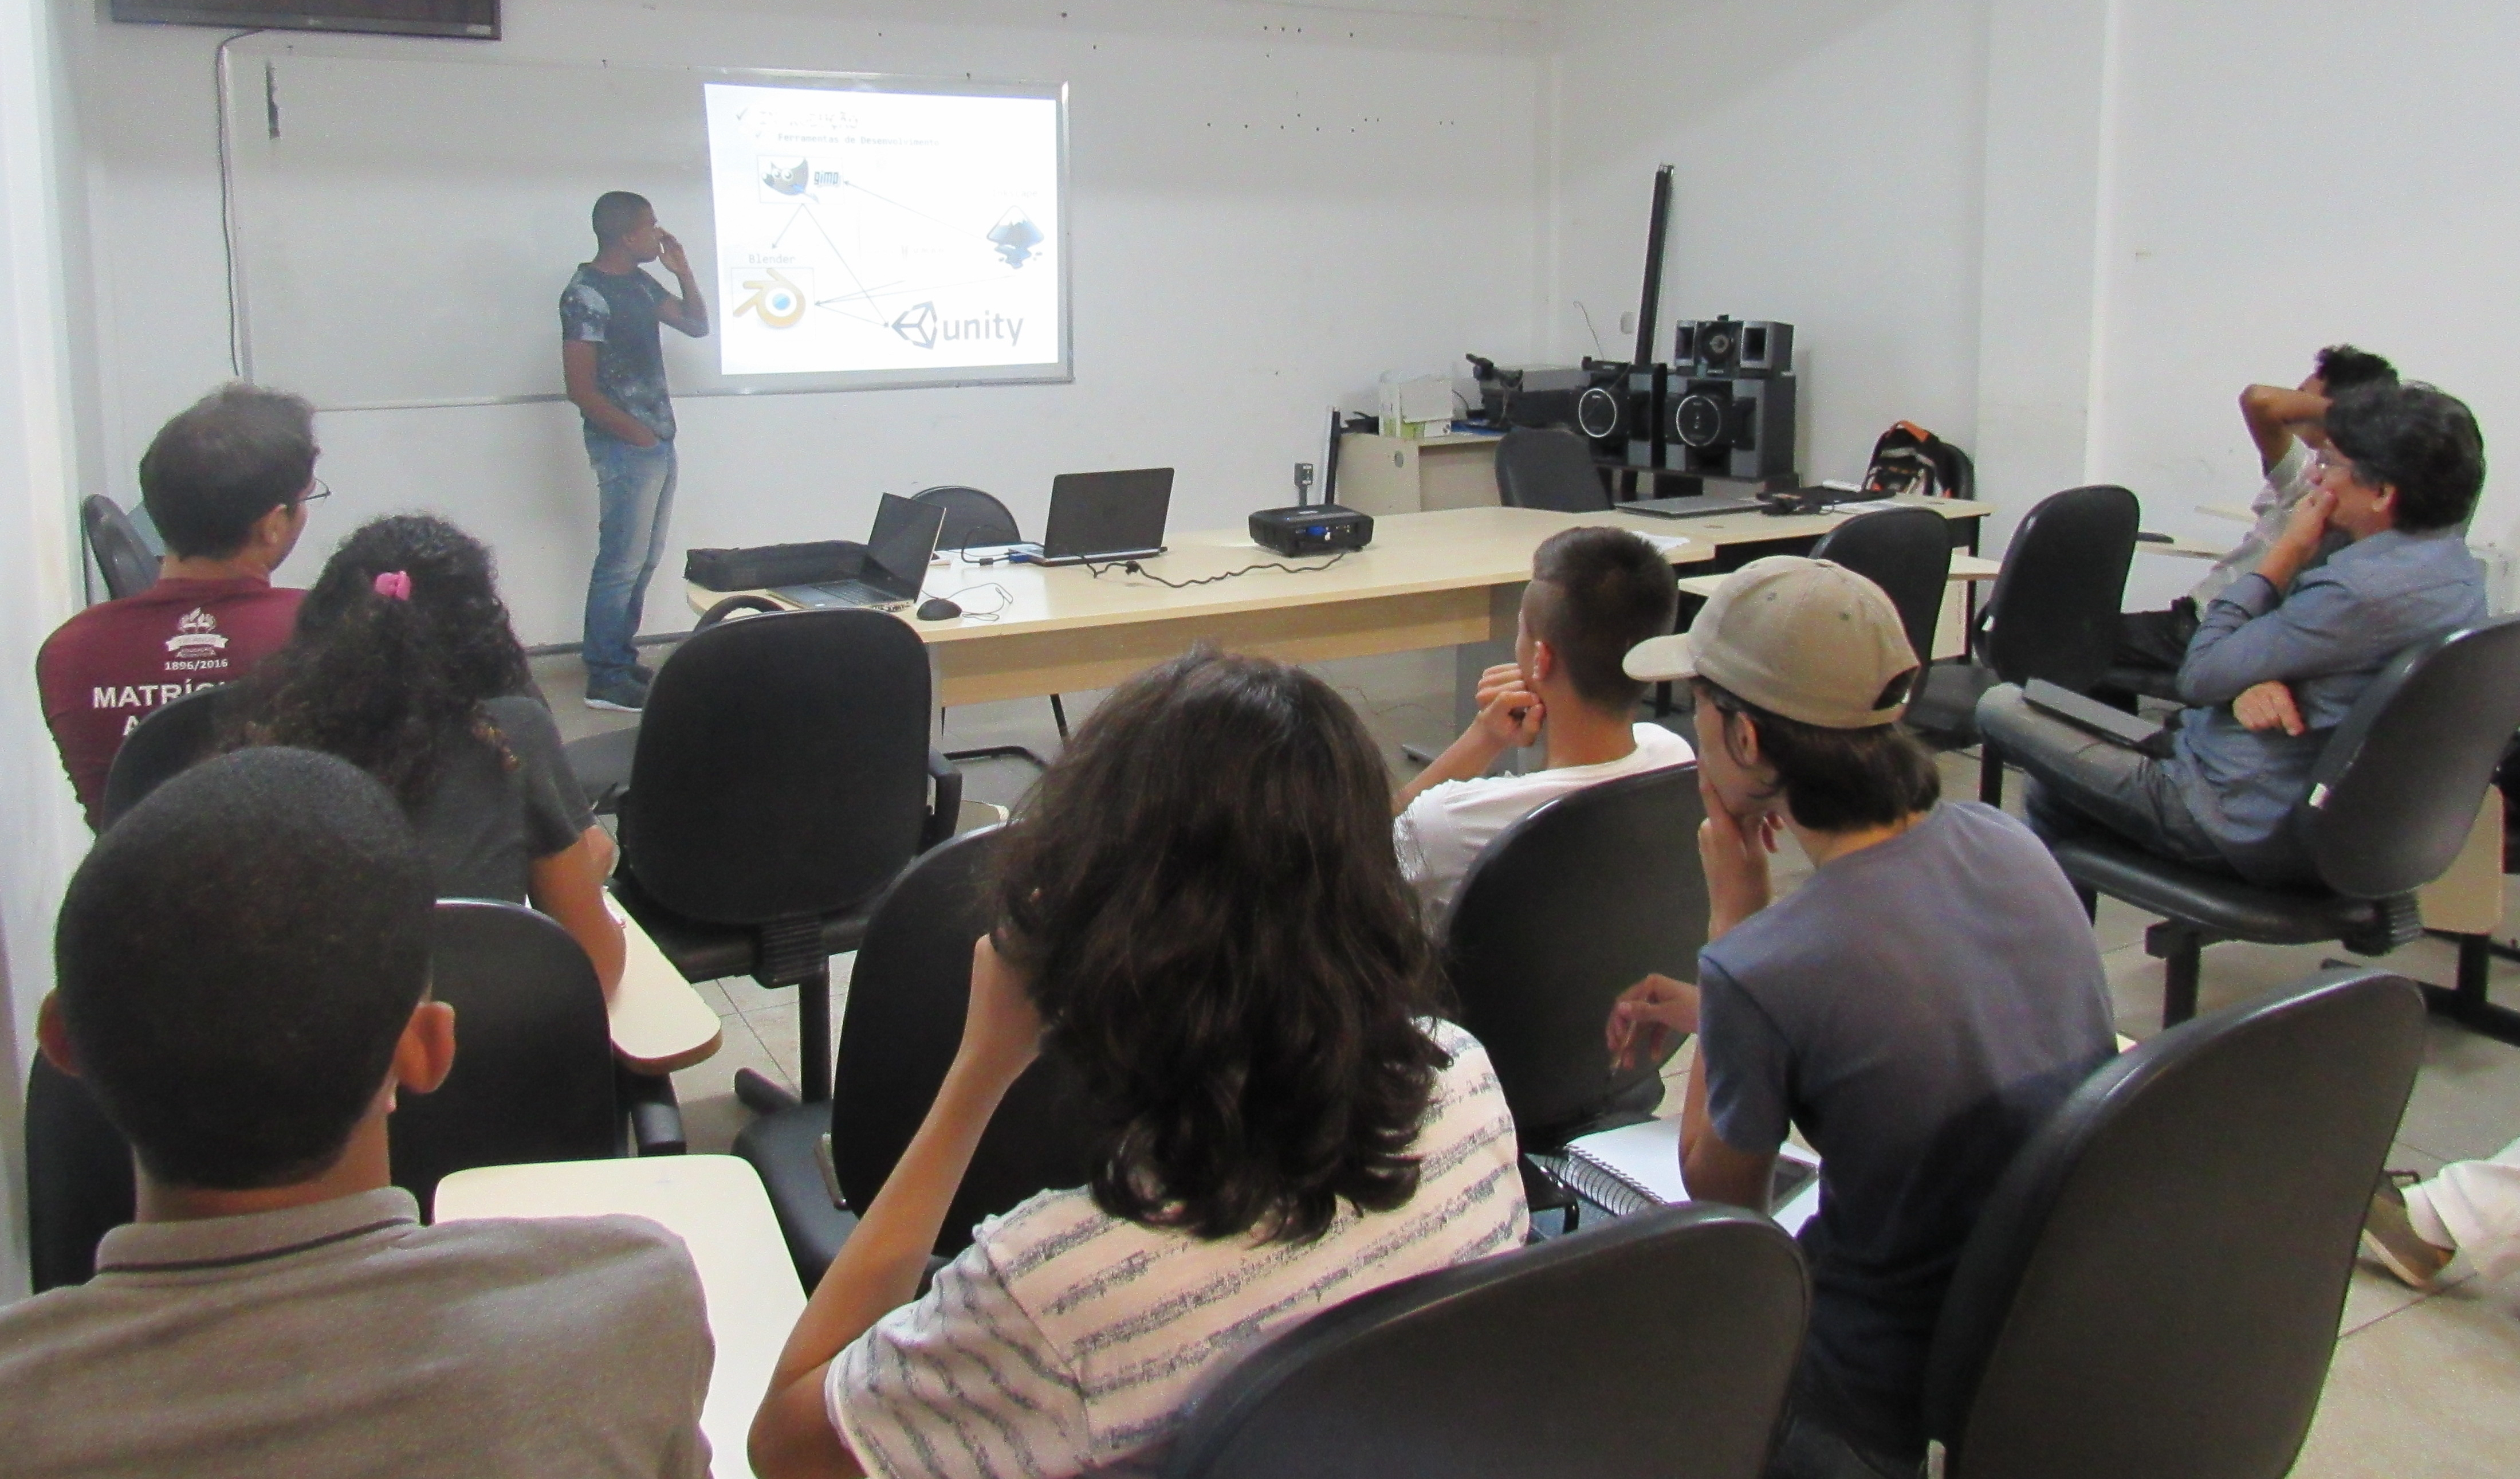
\includegraphics[width=0.7\textwidth]{figuras/workshop_alunos.jpg}
	\label{fig:palestra-jogos}
	{\fonte{O Autor (2018)}}
\end{figure}

\begin{figure}[H]
	\centering
	\caption{Aluno testando o jogo}
	\includegraphics[width=0.62\textwidth]{figuras/aluno_teste.jpg}
	\label{fig:avaliacao-aluno}
	{\fonte{O Autor (2018)}}
\end{figure} % Revisão de Literatura
	% % CRONOGRAMA DE ATIVIDADES------------------------------------------------------------------

\chapter{CRONOGRAMA DE ATIVIDADES}
\label{chap:cronograma}

Este capítulo apresenta o cronograma de atividades do projeto, destacando os passos necessários para o alcance dos objetivos apresentados.

\begin{table}[htb]
	\IBGEtab{%
		\caption{Cronograma de Atividades do Projeto}%
		\label{tab:cronograma}
	}{%
		\begin{tabular}{c}
			\includegraphics[scale=1]{figuras/cronograma.png}
		\end{tabular}%
	}{%
		\fonte{Autoria própria}%
	}
\end{table}
 
 % Cronograma de Atividades
	% CONCLUSÃO--------------------------------------------------------------------

\chapter{CONSIDERAÇÕES FINAIS}
\label{chap:conclusao}

Este trabalho descreveu o projeto e implementação de partes componentes de um jogo de plataforma \textit{2D} sobre um acontecimento recente da história brasileira, a Guerrilha do Araguaia. Foi apresentado o processo de desenvolvimento de quatro \textit{cutscenes}, uma em \textit{3D} e três em \textit{2D}, e quatro missões. Duas missões relacionadas a primeira fase do jogo, e duas a segunda fase. Foi formada uma equipe interdisciplinar com profissionais da área de história e da área de produção de games. Inicialmente a equipe passou por um processo de ambientação sobre o assunto a ser relatado na forma de um game, e trabalhou de forma colaborativa na escolha do estilo do jogo e na definição do seu enredo e roteiro. Os resultados, até aqui alcançados com a finalização das duas fases são animadores e motivadores. É um jogo que une diversão e que ao mesmo tempo instrui não só sobre os acontecimentos históricos, mas também sobre a flora e fauna do palco dos acontecimentos.

A distribuição do jogo foi feita em dois aplicativos. O primeiro aplicativo, que se refere a primeira fase do jogo, onde o período de ambientação na região é retratado. E o segundo aplicativo, que mostra o relacionamento com a população e treinamento dos guerrilheiros; e o conflito armado (tabela \ref{tab:enrrotmis}).

Inicialmente, o primeiro aplicativo foi construído na plataforma \textit{desktop} e testado com boa aceitação nas turmas do primeiro ano do ensino médio de um colégio particular. A equipe tentou levar esta versão, também para escolas públicas, mas encontrou dificuldades devido a baixa qualidade dos computadores, tanto de hardware como de software, onde usam um sistema operacional \textit{Linux} antiquado e principalmente a falta de manutenção torna muito difícil a utilização do jogo por parte de alunos e professores.

Diante disso, a equipe constatou que a grande maioria dos alunos das escolas públicas possuem aparelhos celulares com capacidade suficiente para rodar jogos no estilo plataforma \textit{2D}, e decidiu que o jogo seria distribuído para \textit{mobile} \textit{(Android)}, por ser a mais popular entre os alunos das escolas públicas. Assim, os dois aplicativos estão construídos para dispositivos móveis, disponíveis para \textit{download} em \url{https://lage.unifesspa.edu.br/baixar-games-main.html}. Acredita-se que, o que foi construído neste trabalho reúne material suficiente para ser apresentado como um game educativo lúdico sobre um fato histórico tão pouco conhecido por professores e alunos.

\section{Trabalhos Futuros}

Como trabalho futuro, sugere-se a realização da avaliação com alunos (descrita na seção \ref{sec:desenvolvimento}) em algumas escolas do município de Marabá-PA, para evidenciar quantitativamente a receptividade do jogo por parte dos envolvidos, tal como a experiência destes, por meio da aplicação de um questionário extraído de um modelo para avaliação de jogos educacionais, descrito em \citeonline{bib:savi2011}.

\section{Artigos Publicados}

\begin{itemize}
	\item OLIVEIRA, Gilberto P.; RESPLANDES, Denison S.; SILVA, Caique; SOUZA, Adriano; ARAÚJO, Tiago de S.; LUIZ, Janailson M.; RIBEIRO, Manoel F. Guerrilha do Araguaia: A atuação do guerrilheiro Osvaldão em um Jogo de Plataforma que conta um episódio histórico Pouco Conhecido. Publicado no $XVI$ SBGames -- Simpósio Brasileiro de Jogos e Entretenimento Digital, realizado em novembro de $2017$, em Curitiba-PR (Apêndice \ref*{chap:apendiceA} e Anexo \ref*{chap:anexoA}).
	
	% \item OLIVEIRA, Gilberto P.; RESPLANDES, Denison S.; RIBEIRO, Manoel F.; LUIZ, Janailson M.; SOBRAL, Marcos; NOGUEIRA, Felipe. Araguaia -- A Saga de Osvaldão: um jogo educativo sobre a Guerrilha do Araguaia para a plataforma \textit{Android}. Publicado no SBIE $2018$, $XXIX$ Simpósio Brasileiro de Informática na Educação (SBIE -- Trilha $2$: Jogos, simulação, gamificação, robótica, realidade virtual e mundos virtuais para promoção da aprendizagem), com aceite previsto para meados de agosto de $2018$.
\end{itemize}

 % Considerações Finais
	
	\postextual
	%
% Documento: Referências Bibliográficas
%

\bibliography{base-referencias}
\bibliographystyle{abntex2-alf} % Define o estilo ABNT para formatar a lista de referências % Referências
	% APÊNDICES--------------------------------------------------------------------

\begin{apendicesenv}
\partapendices

% Primeiro apêndice ------------------------------------------------------------
\chapter{Guerrilha do Araguaia: A Atuação do Guerrilheiro Osvaldão em um Jogo de  Plataforma que conta  um Episódio Histórico Pouco Conhecido}

\label{chap:apendiceA}

\includepdf[pages=-]{figuras/175172.pdf}

\end{apendicesenv}
 % Apêndices
	% ANEXO------------------------------------------------------------------------

\begin{anexosenv}
\partanexos

% Primeiro anexo ---------------------------------------------------------------
\chapter{Certificado de Publicação no XVI Simpósio Brasileiro de Games e Entretenimento Digital SBGames 2017}

\label{chap:anexoA}

\includepdf[pages=-, angle=90]{figuras/SBGames17.pdf}

\end{anexosenv}
 % Anexos
			
\end{document}
